\documentclass[10pt]{article}
\usepackage[T1]{fontenc}
\usepackage[utf8]{inputenc}
%\DeclareUnicodeCharacter{00A0}{ }
\usepackage[adobe-utopia]{mathdesign}

\usepackage{amsmath}
\usepackage[francais]{babel}
\usepackage[dvips]{graphicx}
%\usepackage{here}
\usepackage{framed}
\usepackage[normalem]{ulem}
\usepackage{fancyhdr}
\usepackage{titlesec}
\usepackage{vmargin}

\usepackage{amsmath}
\usepackage{ifthen}
\usepackage{multirow}
\usepackage{multicol} % Portions de texte en colonnes

%\usepackage{xltxtra} % Logo XeLaTeX
%\usepackage{pst-solides3d}
\usepackage{color}
%\usepackage{colortbl}
\usepackage{titletoc} % Pour la mise en forme de la table des matières

%\usepackage[crop=off]{auto-pst-pdf}
%\usepackage{bclogo}


%\usepackage{longtable}
%\usepackage{flafter}%floatants après la référence
%\usepackage{pst-solides3d}
%\usepackage{pstricks}
%\usepackage{minitoc}
%\setcounter{minitocdepth}{4}
%\usepackage{draftcopy}% "Brouillon"
%\usepackage{floatflt}
%\usepackage{psfrag}
%\usepackage{listings} % Permet d'insérer du code de programmation
%\usepackage{lmodern}
%\usepackage[adobe-utopia,uppercase=upright,greeklowercase=upright]{mathdesign}
%\usepackage{minionpro}
%\usepackage{pifont}
%\usepackage{amssymb}
%\usepackage[francais]{varioref}

\setmarginsrb{1.5cm}{1cm}{1cm}{1.5cm}{1cm}{1cm}{1cm}{1cm}

\definecolor{gris25}{gray}{0.75}
\definecolor{bleu}{RGB}{18,33,98}
\definecolor{bleuf}{RGB}{42,94,171}
\definecolor{bleuc}{RGB}{231,239,247}
\definecolor{rougef}{RGB}{185,18,27}
\definecolor{rougec}{RGB}{255,230,231}
\definecolor{vertf}{RGB}{103,126,82}
\definecolor{vertc}{RGB}{220,255,191}
\definecolor{violetf}{RGB}{112,48,160}
\definecolor{violetc}{RGB}{230,224,236}
\definecolor{jaunec}{RGB}{220,255,191}
%\usepackage{algorithm}
%\usepackage{algorithmic}
\usepackage[french]{algorithm2e}

\SetKwBlock{Fonction}{Début Fonction}{Fin Fonction}
\SetKwComment{Comment}{start}{end}
% Python sources

\usepackage{listings}
\lstloadlanguages{R}   % pour regler les pb d accent utf8 dans les codes
\lstset{language=R} % pour regler les pb d accent utf8 dans les codes

\usepackage{textcomp}
\usepackage{setspace}
%\usepackage{palatino}

%\usepackage{color}
\definecolor{Bleu}{rgb}{0.1,0.1,1.0}
\definecolor{Noir}{rgb}{0,0,0}
\definecolor{Grau}{rgb}{0.5,0.5,0.5}
\definecolor{DunkelGrau}{rgb}{0.15,0.15,0.15}
\definecolor{Hellbraun}{rgb}{0.5,0.25,0.0}
\definecolor{Magenta}{rgb}{1.0,0.0,1.0}
\definecolor{Gris}{gray}{0.5}
\definecolor{Vert}{rgb}{0,0.5,0}
\definecolor{SourceHintergrund}{rgb}{1,1.0,0.95}


%
\renewcommand{\lstlistlistingname}{Listings}
\renewcommand{\lstlistingname}{Listing}

\lstnewenvironment{python}[1][]{
\lstset{
%escapeinside={\%*}{*)},
%inputencoding=utf8,   % pour regler les pb d accent utf8 dans les codes
%extendedchars=true,   % pour regler les pb d accent utf8 dans les codes
language=python,
basicstyle=\sffamily\footnotesize, 	
stringstyle=\color{red}, 
showstringspaces=false, 
alsoletter={1234567890},
otherkeywords={\ , \}, \{},
keywordstyle=\color{blue},
emph={access,and,break,class,continue,def,del,elif ,else,
except,exec,finally,for,from,global,if,import,in,i s,
lambda,not,or,pass,print,raise,return,try,while},
emphstyle=\color{black}\bfseries,
emph={[2]True, False, None, self},
emphstyle=[2]\color{green},
emph={[3]from, import, as},
emphstyle=[3]\color{blue},
upquote=true,
columns=flexible, % pour empecher d'avoir un espacement mono
morecomment=[s]{"""}{"""},
commentstyle=\color{Hellbraun}\slshape, 
%emph={[4]1, 2, 3, 4, 5, 6, 7, 8, 9, 0},
emphstyle=[4]\color{blue},
literate=*{:}{{\textcolor{blue}:}}{1}
{=}{{\textcolor{blue}=}}{1}
{-}{{\textcolor{blue}-}}{1}
{+}{{\textcolor{blue}+}}{1}
{*}{{\textcolor{blue}*}}{1}
{!}{{\textcolor{blue}!}}{1}
{(}{{\textcolor{blue}(}}{1}
{)}{{\textcolor{blue})}}{1}
{[}{{\textcolor{blue}[}}{1}
{]}{{\textcolor{blue}]}}{1}
{<}{{\textcolor{blue}<}}{1}
{>}{{\textcolor{blue}>}}{1}
{COMPLETER}{{\textcolor{red}COMPLETER}}{1},
literate=%
            {é}{{\'{e}}}1
            {è}{{\`{e}}}1
            {ê}{{\^{e}}}1
            {ë}{{\¨{e}}}1
            {û}{{\^{u}}}1
            {ù}{{\`{u}}}1
            {â}{{\^{a}}}1
            {à}{{\`{a}}}1
            {î}{{\^{i}}}1
            {ç}{{\c{c}}}1
            {Ç}{{\c{C}}}1
            {É}{{\'{E}}}1
            {Ê}{{\^{E}}}1
            {À}{{\`{A}}}1
            {Â}{{\^{A}}}1
            {Î}{{\^{I}}}1, % pour regler les pb d accent utf8 dans les codes
%framexleftmargin=1mm, framextopmargin=1mm, frame=shadowbox, rulesepcolor=\color{blue},#1
%backgroundcolor=\color{SourceHintergrund}, 
%framexleftmargin=1mm, framexrightmargin=1mm, framextopmargin=1mm, frame=single, framerule=1pt, rulecolor=\color{black},#1
}}{}



\lstnewenvironment{scilab}[1][]{
\lstset{
language=scilab,
basicstyle=\sffamily\footnotesize, 	
stringstyle=\color{red}, 
showstringspaces=false, 
alsoletter={1234567890},
otherkeywords={\ , \}, \{},
keywordstyle=\color{blue},
emph={access,and,break,class,continue,def,del,elif ,else,
except,exec,finally,for,from,global,if,import,in,i s,
lambda,not,or,pass,print,raise,return,try,while,Debut},
emphstyle=\color{black}\bfseries,
emph={[2]True, False, None, self},
emphstyle=[2]\color{green},
emph={[3]from, import, as},
emphstyle=[3]\color{blue},
upquote=true,
columns=flexible, % pour empecher d'avoir un espacement mono
morecomment=[s]{"""}{"""},
commentstyle=\color{Hellbraun}\slshape, 
%emph={[4]1, 2, 3, 4, 5, 6, 7, 8, 9, 0},
emphstyle=[4]\color{blue},
literate=*{:}{{\textcolor{blue}:}}{1}
{=}{{\textcolor{blue}=}}{1}
{-}{{\textcolor{blue}-}}{1}
{+}{{\textcolor{blue}+}}{1}
{*}{{\textcolor{blue}*}}{1}
{!}{{\textcolor{blue}!}}{1}
{(}{{\textcolor{blue}(}}{1}
{)}{{\textcolor{blue})}}{1}
{[}{{\textcolor{blue}[}}{1}
{]}{{\textcolor{blue}]}}{1}
{<}{{\textcolor{blue}<}}{1}
{>}{{\textcolor{blue}>}}{1},
%framexleftmargin=1mm, framextopmargin=1mm, frame=shadowbox, rulesepcolor=\color{blue},#1
%backgroundcolor=\color{SourceHintergrund}, 
%framexleftmargin=1mm, framexrightmargin=1mm, framextopmargin=1mm, frame=single, framerule=1pt, rulecolor=\color{black},#1
}}{}


\lstdefinestyle{stylepython}{%
escapeinside={\%*}{*)},
inputencoding=utf8,   % pour regler les pb d accent utf8 dans les codes
extendedchars=true,   % pour regler les pb d accent utf8 dans les codes
language=python,
basicstyle=\sffamily\footnotesize, 	
stringstyle=\color{red}, 
showstringspaces=false, 
alsoletter={1234567890},
otherkeywords={\ , \}, \{},
keywordstyle=\color{blue},
emph={access,and,break,class,continue,def,del,elif ,else,
except,exec,finally,for,from,global,if,import,in,i s,
lambda,not,or,pass,print,raise,return,try,while},
emphstyle=\color{black}\bfseries,
emph={[2]True, False, None, self},
emphstyle=[2]\color{green},
emph={[3]from, import, as},
emphstyle=[3]\color{blue},
upquote=true,
columns=flexible, % pour empecher d'avoir un espacement mono
morecomment=[s]{"""}{"""},
commentstyle=\color{Hellbraun}\slshape, 
%emph={[4]1, 2, 3, 4, 5, 6, 7, 8, 9, 0},
emphstyle=[4]\color{blue},
literate=*{:}{{\textcolor{blue}:}}{1}
{=}{{\textcolor{blue}=}}{1}
{-}{{\textcolor{blue}-}}{1}
{+}{{\textcolor{blue}+}}{1}
{*}{{\textcolor{blue}*}}{1}
{!}{{\textcolor{blue}!}}{1}
{(}{{\textcolor{blue}(}}{1}
{)}{{\textcolor{blue})}}{1}
{[}{{\textcolor{blue}[}}{1}
{]}{{\textcolor{blue}]}}{1}
{<}{{\textcolor{blue}<}}{1}
{>}{{\textcolor{blue}>}}{1}
{COMPLETER}{{\textcolor{red}COMPLETER}}{1},
literate=%
            {é}{{\'{e}}}1
            {è}{{\`{e}}}1
            {ê}{{\^{e}}}1
            {ë}{{\¨{e}}}1
            {û}{{\^{u}}}1
            {ù}{{\`{u}}}1
            {â}{{\^{a}}}1
            {à}{{\`{a}}}1
            {î}{{\^{i}}}1
            {ç}{{\c{c}}}1
            {Ç}{{\c{C}}}1
            {É}{{\'{E}}}1
            {Ê}{{\^{E}}}1
            {À}{{\`{A}}}1
            {Â}{{\^{A}}}1
            {Î}{{\^{I}}}1,
%numbers=left,                    % where to put the line-numbers; possible values are (none, left, right)
%numbersep=5pt,                   % how far the line-numbers are from the code
%numberstyle=\tiny\color{mygray}, % the style that is used for the line-numbers
}

%
%\renewcommand{\algorithmicrequire} {\textbf{\textsc{Entrées:}}}
%\renewcommand{\algorithmicensure}  {\textbf{\textsc{Sorties:}}}
%\renewcommand{\algorithmicwhile}   {\textbf{tantque}}
%\renewcommand{\algorithmicdo}      {\textbf{faire}}
%\renewcommand{\algorithmicendwhile}{\textbf{fin tantque}}
%\renewcommand{\algorithmicend}     {\textbf{fin}}
%\renewcommand{\algorithmicif}      {\textbf{si}}
%\renewcommand{\algorithmicendif}   {\textbf{finsi}}
%\renewcommand{\algorithmicelse}    {\textbf{sinon}}
%\renewcommand{\algorithmicthen}    {\textbf{alors}}
%\renewcommand{\algorithmicfor}     {\textbf{pour}}
%\renewcommand{\algorithmicforall}  {\textbf{pour tout}}
%\renewcommand{\algorithmicdo}      {\textbf{faire}}
%\renewcommand{\algorithmicendfor}  {\textbf{fin pour}}
%\renewcommand{\algorithmicloop}    {\textbf{boucler}}
%\renewcommand{\algorithmicendloop} {\textbf{fin boucle}}
%\renewcommand{\algorithmicrepeat}  {\textbf{répéter}}
%\renewcommand{\algorithmicuntil}   {\textbf{jusqu'à}}

\lstnewenvironment{termi}[1][]{
\lstset{
language=scilab,
basicstyle=\sffamily\footnotesize, 	
stringstyle=\color{red}, 
showstringspaces=false, 
alsoletter={1234567890},
otherkeywords={\ , \}, \{},
keywordstyle=\color{blue},
emph={access,and,break,class,continue,def,del,elif ,else,
except,exec,finally,for,from,global,if,import,in,i s,
lambda,not,or,pass,print,raise,return,try,while,Debut},
emphstyle=\color{black}\bfseries,
emph={[2]True, False, None, self},
emphstyle=[2]\color{green},
emph={[3]from, import, as},
emphstyle=[3]\color{blue},
upquote=true,
columns=flexible, % pour empecher d'avoir un espacement mono
morecomment=[s]{"""}{"""},
commentstyle=\color{Hellbraun}\slshape, 
%emph={[4]1, 2, 3, 4, 5, 6, 7, 8, 9, 0},
emphstyle=[4]\color{blue},
literate=*{:}{{\textcolor{blue}:}}{1}
{=}{{\textcolor{blue}=}}{1}
{-}{{\textcolor{blue}-}}{1}
{+}{{\textcolor{blue}+}}{1}
{*}{{\textcolor{blue}*}}{1}
{!}{{\textcolor{blue}!}}{1}
{(}{{\textcolor{blue}(}}{1}
{)}{{\textcolor{blue})}}{1}
{[}{{\textcolor{blue}[}}{1}
{]}{{\textcolor{blue}]}}{1}
{<}{{\textcolor{blue}<}}{1}
{>}{{\textcolor{blue}>}}{1},
%framexleftmargin=1mm, framextopmargin=1mm, frame=shadowbox, rulesepcolor=\color{blue},#1
%backgroundcolor=\color{SourceHintergrund}, 
%framexleftmargin=1mm, framexrightmargin=1mm, framextopmargin=1mm, frame=single, framerule=1pt, rulecolor=\color{black},#1
}}{}


%
%\renewcommand{\algorithmicrequire} {\textbf{\textsc{Entrées:}}}
%\renewcommand{\algorithmicensure}  {\textbf{\textsc{Sorties:}}}
%\renewcommand{\algorithmicwhile}   {\textbf{tantque}}
%\renewcommand{\algorithmicdo}      {\textbf{faire}}
%\renewcommand{\algorithmicendwhile}{\textbf{fin tantque}}
%\renewcommand{\algorithmicend}     {\textbf{fin}}
%\renewcommand{\algorithmicif}      {\textbf{si}}
%\renewcommand{\algorithmicendif}   {\textbf{finsi}}
%\renewcommand{\algorithmicelse}    {\textbf{sinon}}
%\renewcommand{\algorithmicthen}    {\textbf{alors}}
%\renewcommand{\algorithmicfor}     {\textbf{pour}}
%\renewcommand{\algorithmicforall}  {\textbf{pour tout}}
%\renewcommand{\algorithmicdo}      {\textbf{faire}}
%\renewcommand{\algorithmicendfor}  {\textbf{fin pour}}
%\renewcommand{\algorithmicloop}    {\textbf{boucler}}
%\renewcommand{\algorithmicendloop} {\textbf{fin boucle}}
%\renewcommand{\algorithmicrepeat}  {\textbf{répéter}}
%\renewcommand{\algorithmicuntil}   {\textbf{jusqu'à}}
%%%%%%%%%%%%
% Définition des vecteurs 
%%%%%%%%%%%%
 \newcommand{\vect}[1]{\overrightarrow{#1}}
\newcommand{\axe}[2]{\left(#1,\vect{#2}\right)}

\newcommand{\rep}[1]{\mathcal{R}_{#1}}
\newcommand{\vx}[1]{\vect{x_{#1}}}
\newcommand{\vy}[1]{\vect{y_{#1}}}
\newcommand{\vz}[1]{\vect{z_{#1}}}

%%%%%%%%%%%%
% Définition des torseurs 
%%%%%%%%%%%%

 \newcommand{\torseur}[1]{%
\left\{{#1}\right\}
}

\newcommand{\torseurcin}[3]{%
\left\{\mathcal{#1} \left(#2/#3 \right) \right\}
}

\newcommand{\torseurstat}[3]{%
\left\{\mathcal{#1} \left(#2\rightarrow #3 \right) \right\}
}

 \newcommand{\torseurc}[8]{%
%\left\{#1 \right\}=
\left\{
{#1}
\right\}
 = 
\left\{%
\begin{array}{cc}%
{#2} & {#5}\\%
{#3} & {#6}\\%
{#4} & {#7}\\%
\end{array}%
\right\}_{#8}%
}

 \newcommand{\torseurcol}[7]{
\left\{%
\begin{array}{cc}%
{#1} & {#4}\\%
{#2} & {#5}\\%
{#3} & {#6}\\%
\end{array}%
\right\}_{#7}%
}

 \newcommand{\torseurl}[3]{%
%\left\{\mathcal{#1}\right\}_{#2}=%
\left\{%
\begin{array}{l}%
{#1} \\%
{#2} %
\end{array}%
\right\}_{#3}%
}

 \newcommand{\vectv}[3]{%
\vect{V\left( {#1} \in {#2}/{#3}\right)}
}


\newcommand{\vectf}[2]{%
\vect{R\left( {#1} \rightarrow {#2}\right)}
}

\newcommand{\vectm}[3]{%
\vect{\mathcal{M}\left( {#1}, {#2} \rightarrow {#3}\right)}
}


 \newcommand{\vectg}[3]{%
\vect{\Gamma \left( {#1} \in {#2}/{#3}\right)}
}

 \newcommand{\vecto}[2]{%
\vect{\Omega\left( {#1}/{#2}\right)}
}
% }$$\left\{\mathcal{#1} \right\}_{#2} =%
% \left\{%
% \begin{array}{c}%
%  #3 \\%
%  #4 %
% \end{array}%
% \right\}_{#5}}
\setcounter{tocdepth}{2}
% \mtcselectlanguage{french} 


%  ------------------------------------------
% | Modification du formatage des sections : | 
%  ------------------------------------------

% Grands titres :
% ---------------

\newcommand{\titre}[1]{%
\begin{center}
      \bigskip
      \rule{\textwidth}{1pt}
      \par\vspace{0.1cm}
      
      \textbf{\large #1}
      \par\rule{\textwidth}{1pt}
    \end{center}
    \bigskip
  }

% Supprime le numéro du chapitre dans la numérotation des sections:
% -----------------------------------------------------------------
\makeatletter
\renewcommand{\thesection}{\@arabic\c@section}
\makeatother


% \titleformat{\chapter}[display]
% {\normalfont\Large\filcenter}
% {}
% {1pc}
% {\titlerule[1pt]
%   \vspace{1pc}%
%   \Huge}[\vspace{1ex}%
% \titlerule]


%%%% Chapitres Comme PY Pechard %%%%%%%%%
% numéro du chapitre
\DeclareFixedFont{\chapnumfont}{OT1}{phv}{b}{n}{80pt}
% pour le mot « Chapitre »
\DeclareFixedFont{\chapchapfont}{OT1}{phv}{m}{it}{40pt}
% pour le titre
\DeclareFixedFont{\chaptitfont}{T1}{phv}{b}{n}{25pt}

\definecolor{gris}{gray}{0.75}
\titleformat{\chapter}[display]%
	{\sffamily}%
	{\filleft\chapchapfont\color{gris}\chaptertitlename\
	\\
	\vspace{12pt}
	\chapnumfont\thechapter}%
	{16pt}%
	{\filleft\chaptitfont}%
	[\vspace{6pt}\titlerule\titlerule\titlerule]

%%%%  Fin Chapitres Comme PY Pechard %%%%%%%%%


% Section, subsection, subsubsection sans serifs :
% % ----------------------------------------------

% \makeatletter
% \renewcommand{\section}{\@startsection{section}{0}{0mm}%
% {\baselineskip}{.3\baselineskip}%
% {\normalfont\sffamily\Large\textbf}}%
% \makeatother

\makeatletter
\renewcommand{\@seccntformat}[1]{{\textcolor{bleu}{\csname
the#1\endcsname}\hspace{0.5em}}}
\makeatother

\makeatletter
\renewcommand{\section}{\@startsection{section}{1}{\z@}%
                       {-4ex \@plus -1ex \@minus -.4ex}%
                       {1ex \@plus.2ex }%
                       {\normalfont\Large\sffamily\bfseries}}%
\makeatother
 
\makeatletter
\renewcommand{\subsection}{\@startsection {subsection}{2}{\z@}
                          {-3ex \@plus -0.1ex \@minus -.4ex}%
                          {0.5ex \@plus.2ex }%
                          {\normalfont\large\sffamily\bfseries}}
\makeatother
 
\makeatletter
\renewcommand{\subsubsection}{\@startsection {subsubsection}{3}{\z@}
                          {-2ex \@plus -0.1ex \@minus -.2ex}%
                          {0.2ex \@plus.2ex }%
                          {\normalfont\large\sffamily\bfseries}}
\makeatother
 
\makeatletter             
\renewcommand{\paragraph}{\@startsection{paragraph}{4}{\z@}%
                                    {-2ex \@plus-.2ex \@minus .2ex}%
                                    {0.1ex}%               
{\normalfont\sffamily\bfseries}}
\makeatother
 
 
\makeatletter             
\renewcommand{\subparagraph}{\@startsection{subparagraph}{5}{\z@}%
                                    {-2ex \@plus-.2ex \@minus .2ex}%
                                    {0.1ex}%               
{\normalfont\bfseries Question }}
\makeatother
\renewcommand{\thesubparagraph}{\arabic{subparagraph}} 
\makeatletter

\setcounter{secnumdepth}{5}





% Formatage de la table des matières 
% Paquets nécessaires : titletoc ?

% Chapitre spéciaux écrits dans un nombre cerclé dans la table des matières.
\titlecontents{chapter}[+3pc]
  {\addvspace{10pt}\sffamily\bfseries}
{\contentslabel[{\pscirclebox[fillstyle=solid,fillcolor=gray!25,
linecolor=gray!25,framesep=4pt]{\textcolor{white}{\thecontentslabel}}}]{2.5pc}}
  {}
  {\dotfill \normalfont\thecontentspage\ }

\titlecontents{section}[3pc]
  {\addvspace{2pt}\sffamily}
  {\contentslabel[\thecontentslabel]{1.8pc}}
  {}
  {\dotfill \normalfont\thecontentspage\ }

\titlecontents{subsection}[5pc]
  {\addvspace{2pt}\sffamily}
  {\contentslabel[\thecontentslabel]{1.8pc}}
  {}
  {\dotfill \normalfont\thecontentspage\ }

\titlecontents{subsubsection}[8pc]
  {\addvspace{2pt}\sffamily}
  {\contentslabel[\thecontentslabel]{3pc}}
  {}
  {\dotfill \normalfont\thecontentspage\ }
%{\;\titlerule\;\normalfont\thecontentspage\ }

\titlecontents{paragraph}[9pc]
  {\addvspace{2pt}\sffamily}
  {\contentslabel[\thecontentslabel]{3.5pc}}
  {}
  {\dotfill \normalfont\thecontentspage\ }

%pour avoir l indentation dans minipage
\newdimen\oldparindent\oldparindent=\parindent

\makeatletter
\def\@iiiminipage#1#2[#3]#4{%
  \noindent
  \leavevmode
  \@pboxswfalse
  \setlength\@tempdima{#4}%
  \def\@mpargs{{#1}{#2}[#3]{#4}}%
  \setbox\@tempboxa\vbox\bgroup
    \color@begingroup
      \hsize\@tempdima
      \textwidth\hsize \columnwidth\hsize
      \@parboxrestore
      \parindent=\oldparindent
      \def\@mpfn{mpfootnote}\def\thempfn{\thempfootnote}\c@mpfootnote\z@
      \let\@footnotetext\@mpfootnotetext
      \let\@listdepth\@mplistdepth \@mplistdepth\z@
      \@minipagerestore
      \@setminipage}
\makeatother

% Paquets requis : 

\definecolor{gris25}{gray}{0.75}
\definecolor{bleu}{RGB}{18,33,98}
\definecolor{bleuf}{RGB}{42,94,171}
\definecolor{bleuc}{RGB}{231,239,247}
\definecolor{rougef}{RGB}{185,18,27}
\definecolor{rougec}{RGB}{255,230,231}
\definecolor{vertf}{RGB}{103,126,82}
\definecolor{vertc}{RGB}{220,255,191}
\definecolor{violetf}{RGB}{112,48,160}
\definecolor{violetc}{RGB}{230,224,236}
\definecolor{jaunec}{RGB}{220,255,191}



\newenvironment{corrige}[1][\hsize]%
{%
    \def\FrameCommand%
    {%
\rotatebox{90}{\textit{\textsf{Corrigé}}} 
        {\color{violetf}\vrule width 3pt}%
        \hspace{0pt}%must no space.
        \fboxsep=\FrameSep\colorbox{violetc}%
    }%
    \MakeFramed{\hsize #1 \advance\hsize-\width\FrameRestore}%
}%
{\endMakeFramed}%

\newenvironment{sci}[1][\hsize]%
{%
    \def\FrameCommand%
    {%
%\rotatebox{90}{\textit{\textsf{Scilab}}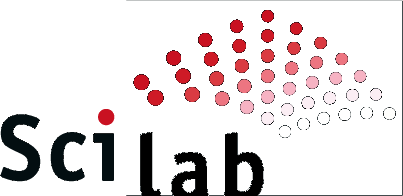
\includegraphics[height=.8cm]{png/logo_scilab}} 
\rotatebox{90}{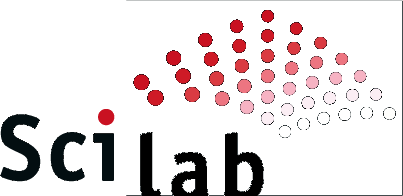
\includegraphics[height=.6cm]{png/logo_scilab}} 
        {\color{violetf}\vrule width 3pt}%
        \hspace{0pt}%must no space.
        \fboxsep=\FrameSep\colorbox{violetc}%
    }%
    \MakeFramed{\hsize #1 \advance\hsize-\width\FrameRestore}%
}%
{\endMakeFramed}%

\newenvironment{pseudo}[1][\hsize]%
{%
    \def\FrameCommand%
    {%
\rotatebox{90}{\textit{\textsf{Pseudo Code}}} 
        {\color{violetf}\vrule width 3pt}%
        \hspace{0pt}%must no space.
        \fboxsep=\FrameSep\colorbox{violetc}%
    }%
    \MakeFramed{\hsize #1 \advance\hsize-\width\FrameRestore}%
}%
{\endMakeFramed}%

\newenvironment{py}[1][\hsize]%
{%
    \def\FrameCommand%
    {%
%\rotatebox{90}{\textit{\textsf{Python}}} 
\rotatebox{90}{
\includegraphics[height=.6cm]{png/logo_python}} 
        {\color{violetf}\vrule width 3pt}%
        \hspace{0pt}%must no space.
        \fboxsep=\FrameSep\colorbox{violetc}%
    }%
    \MakeFramed{\hsize #1 \advance\hsize-\width\FrameRestore}%
}%
{\endMakeFramed}%


\newenvironment{term}[1][\hsize]%
{%
    \def\FrameCommand%
    {%
\rotatebox{90}{\textit{\textsf{Terminal}}} 
        {\color{violetf}\vrule width 3pt}%
        \hspace{0pt}%must no space.
        \fboxsep=\FrameSep\colorbox{violetc}%
    }%
    \MakeFramed{\hsize #1 \advance\hsize-\width\FrameRestore}%
}%
{\endMakeFramed}%


\newenvironment{rem}[1][\hsize]%
{%
    \def\FrameCommand
    {%
\rotatebox{90}{\textit{\textsf{Remarque}}} 
        {\color{bleuf}\vrule width 3pt}%
        \hspace{0pt}%must no space.
        \fboxsep=\FrameSep\colorbox{bleuc}%
    }%
    \MakeFramed{\hsize#1\advance\hsize-\width\FrameRestore}%
}%
{\endMakeFramed}%


\newenvironment{savoir}[1][\hsize]%
{%
    \def\FrameCommand
    {%
\rotatebox{90}{\textit{\textsf{Savoir}}} 
        {\color{bleuf}\vrule width 3pt}%
        \hspace{0pt}%must no space.
        \fboxsep=\FrameSep\colorbox{bleuc}%
    }%
    \MakeFramed{\hsize#1\advance\hsize-\width\FrameRestore}%
}%
{\endMakeFramed}%

\newenvironment{Objectif}[1][\hsize]%
{%
    \def\FrameCommand
    {%
\rotatebox{90}{\textit{\textsf{Objectif}}} 
        {\color{bleuf}\vrule width 3pt}%
        \hspace{0pt}%must no space.
        \fboxsep=\FrameSep\colorbox{bleuc}%
    }%
    \MakeFramed{\hsize#1\advance\hsize-\width\FrameRestore}%
}%
{\endMakeFramed}%

\newenvironment{prob}[1][\hsize]%
{%
    \def\FrameCommand%
    {%
\rotatebox{90}{\textit{\textsf{ Problématique}}} 
        {\color{rougef}\vrule width 3pt}%
        \hspace{0pt}%must no space.
        \fboxsep=\FrameSep\colorbox{rougec}%
    }%
    \MakeFramed{\hsize#1\advance\hsize-\width\FrameRestore}%
}%
{\endMakeFramed}%

\newenvironment{obj}[1][\hsize]%
{%
    \def\FrameCommand%
    {%
\rotatebox{90}{\textit{\textsf{ $\;$}}} 
        {\color{rougef}\vrule width 3pt}%
        \hspace{0pt}%must no space.
        \fboxsep=\FrameSep\colorbox{rougec}%
    }%
    \MakeFramed{\hsize#1\advance\hsize-\width\FrameRestore}%
}%
{\endMakeFramed}%

\newenvironment{defi}[1][\hsize]%
{%
    \def\FrameCommand%
    {%
\rotatebox{90}{\textit{\textsf{Définition\\}}} 
        {\color{bleuf}\vrule width 3pt}%
        \hspace{0pt}%must no space.
        \fboxsep=\FrameSep\colorbox{bleuc}%
    }%
    \MakeFramed{\hsize#1\advance\hsize-\width\FrameRestore}%
}%
{\endMakeFramed}%


\newenvironment{demo}[1][\hsize]%
{%
    \def\FrameCommand%
    {%
\rotatebox{90}{\textit{\textsf{Démonstration\\}}} 
        {\color{bleuf}\vrule width 3pt}%
        \hspace{0pt}%must no space.
        \fboxsep=\FrameSep\colorbox{bleuc}%
    }%
    \MakeFramed{\hsize#1\advance\hsize-\width\FrameRestore}%
}%
{\endMakeFramed}%


\newenvironment{hypo}[1][\hsize]%
{%
    \def\FrameCommand%
    {%
\rotatebox{90}{\textit{\textsf{Hypothèse\\}}} 
        {\color{bleuf}\vrule width 3pt}%
        \hspace{0pt}%must no space.
        \fboxsep=\FrameSep\colorbox{bleuc}%
    }%
    \MakeFramed{\hsize#1\advance\hsize-\width\FrameRestore}%
}%
{\endMakeFramed}%


\newenvironment{prop}[1][\hsize]%
{%
    \def\FrameCommand%
    {%
\rotatebox{90}{\textit{\textsf{Propriété\\}}} 
        {\color{bleuf}\vrule width 3pt}%
        \hspace{0pt}%must no space.
        \fboxsep=\FrameSep\colorbox{bleuc}%
    }%
    \MakeFramed{\hsize#1\advance\hsize-\width\FrameRestore}%
}%
{\endMakeFramed}%

\newenvironment{props}[1][\hsize]%
{%
    \def\FrameCommand%
    {%
\rotatebox{90}{\textit{\textsf{Propriétés\\}}} 
        {\color{bleuf}\vrule width 3pt}%
        \hspace{0pt}%must no space.
        \fboxsep=\FrameSep\colorbox{bleuc}%
    }%
    \MakeFramed{\hsize#1\advance\hsize-\width\FrameRestore}%
}%
{\endMakeFramed}%

\newenvironment{exemple}[1][\hsize]%
{%
    \def\FrameCommand%
    {%
\rotatebox{90}{\textit{\textsf{Exemple\\}}} 
        {\color{vertf}\vrule width 3pt}%
        \hspace{0pt}%must no space.
        \fboxsep=\FrameSep\colorbox{vertc}%
    }%
    \MakeFramed{\hsize#1\advance\hsize-\width\FrameRestore}%
}%
{\endMakeFramed}%

\newenvironment{exercice}[1][\hsize]%
{%
    \def\FrameCommand%
    {%
\rotatebox{90}{\textit{\textsf{Exercice\\}}} 
        {\color{vertf}\vrule width 3pt}%
        \hspace{0pt}%must no space.
        \fboxsep=\FrameSep\colorbox{vertc}%
    }%
    \MakeFramed{\hsize#1\advance\hsize-\width\FrameRestore}%
}%
{\endMakeFramed}%

\newenvironment{Support}[1][\hsize]%
{%
    \def\FrameCommand%
    {%
\rotatebox{90}{\textit{\textsf{Support de cours\\}}} 
        {\color{vertf}\vrule width 3pt}%
        \hspace{0pt}%must no space.
        \fboxsep=\FrameSep\colorbox{jaunec}%
    }%
    \MakeFramed{\hsize#1\advance\hsize-\width\FrameRestore}%
}%
{\endMakeFramed}%

\newenvironment{resultat}[1][\hsize]%
{%
    \def\FrameCommand%
    {%
\rotatebox{90}{\textit{\textsf{Résultat\\}}} 
        {\color{rougef}\vrule width 3pt}%
        \hspace{0pt}%must no space.
        \fboxsep=\FrameSep\colorbox{rougec}%
    }%
    \MakeFramed{\hsize#1\advance\hsize-\width\FrameRestore}%
}%
{\endMakeFramed}%

\newenvironment{methode}[1][\hsize]%
{%
    \def\FrameCommand%
    {%
\rotatebox{90}{\textit{\textsf{Méthode\\}}} 
        {\color{rougef}\vrule width 3pt}%
        \hspace{0pt}%must no space.
        \fboxsep=\FrameSep\colorbox{rougec}%
    }%
    \MakeFramed{\hsize#1\advance\hsize-\width\FrameRestore}%
}%
{\endMakeFramed}%

\newenvironment{theo}[1][\hsize]%
{%
    \def\FrameCommand%
    {%
\rotatebox{90}{\textit{\textsf{Théorème\\}}} 
        {\color{rougef}\vrule width 3pt}%
        \hspace{0pt}%must no space.
        \fboxsep=\FrameSep\colorbox{rougec}%
    }%
    \MakeFramed{\hsize#1\advance\hsize-\width\FrameRestore}%
}%
{\endMakeFramed}%

\newenvironment{warn}[1][\hsize]%
{%
    \def\FrameCommand%
    {%
\rotatebox{90}{\textit{\textsf{Attention\\}}} 
        {\color{rougef}\vrule width 3pt}%
        \hspace{0pt}%must no space.
        \fboxsep=\FrameSep\colorbox{rougec}%
    }%
    \MakeFramed{\hsize#1\advance\hsize-\width\FrameRestore}%
}%
{\endMakeFramed}%
\usepackage{style/schemabloc}
%Si le boolen xp est vrai : compilation pour xabi
%Sinon compilation Damien

\newif\ifprof
\proftrue
%\proffalse

\newif\ifxp
\xptrue
%\xpfalse

\newif\iftd
%\tdtrue
\tdfalse


\usepackage[%
    pdftitle={SLCI - Systèmes du second ordre},
    pdfauthor={Xavier Pessoles},
    colorlinks=true,
    linkcolor=blue,
    citecolor=magenta]{hyperref}


\def\discipline{Sciences Industrielles de l'Ingénieur}
\def\xxtitre{%
\ifxp
CI 2 -- SLCI : Étude du comportement des Systèmes Linéaires Continus Invariants
\else
\fi
}

\def\xxsoustitre{%
\ifxp
Chapitre 5 -- Étude des systèmes fondamentaux du second ordre
\else
\fi}

\def\xxauteur{%
\ifxp
Xavier \textsc{Pessoles}
\else
\fi}

\def\xxpied{%
\ifxp
CI 2 : Étude du comportement des Systèmes Linéaires Continus Invariants\\
Ch. 5 : Étude des systèmes fondamentaux du second ordre -- Cours
\else
\fi}



%---------------------------------------------------------------------------


\begin{document}


\sloppy
\hyphenpenalty 10000


%------------- En tetes et Pieds de Pages ------------

\pagestyle{fancy}
\renewcommand{\headrulewidth}{0pt}
\fancyhead{}
\fancyhead[L]{%
\noindent\begin{minipage}[c]{2.6cm}%

\includegraphics[width=2cm]{png/logo_ptsi.png}%
\end{minipage}}


\fancyhead[C]{\rule{12cm}{.5pt}}


\fancyhead[R]{%
\noindent\begin{minipage}[c]{3cm}
\begin{flushright}
\footnotesize{\textit{\textsf{\discipline}}}%
\end{flushright}
\end{minipage}
}



\fancyhead[C]{\rule{12cm}{.5pt}}

\renewcommand{\footrulewidth}{0.2pt}

\fancyfoot[C]{\footnotesize{\bfseries \thepage}}
\fancyfoot[L]{%
\begin{minipage}[c]{.2\linewidth}
\noindent\footnotesize{{\xxauteur}}
\end{minipage}
}

\fancyfoot[R]{\footnotesize{\xxpied}}

\begin{center}
 \ifthenelse{\boolean{td}}{\Large\textsc{\xxtitre}}{\huge\textsc{\xxtitre}}
\end{center}

\begin{center}
 \ifthenelse{\boolean{td}}{\large\textsc{\xxsoustitre}}{ \LARGE\textsc{\xxsoustitre}}
\end{center}

\vspace{.5cm}









\begin{center}
\begin{tabular}{ccccc}
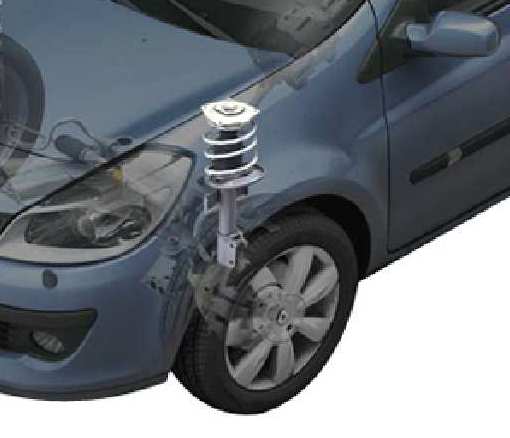
\includegraphics[height=2.5cm]{png/amort1} &&
\includegraphics[height=3.5cm]{png/schema} && 
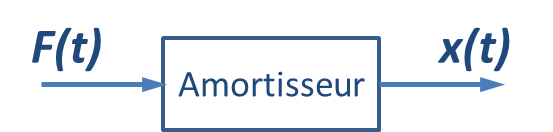
\includegraphics[height=1.5cm]{png/bloc}\\
\textit{Amortisseur d'un véhicule automobile} &&
\textit{Schématisation du mécanisme} &&
\textit{Modélisation par schéma bloc}\\
%\textit{Schéma bloc } \\
\end{tabular}
\end{center}


\vspace{.2cm}


\begin{obj}
\textbf{Problématique :}
\begin{itemize}
\item Le comportement réel de certains systèmes asservis peut se modéliser par des systèmes dits du second ordre. Comment modéliser de tels systèmes ?
%\item Comment modéliser un système complexe multiphysique en utilisant la modélisation en schéma bloc et la modélisation dans le domaine de Laplace ?
%\item Comment déterminer la fonction de transfert d'un système dans le but de prévoir son comportement ?
\end{itemize}
\end{obj}

\begin{savoir}
\textbf{Savoirs :}
\begin{itemize}
\item Mod-C2.3 : Modèles canoniques du second ordre
\begin{itemize}
\item Mod-C2-S1 : Identifier le comportement d’un système pour l’assimiler à un modèle canonique, à partir d’une réponse temporelle 
\item Mod-C2-S2 : Établir un modèle de comportement à partir de relevés expérimentaux
%\item Mod-C2-S3 : On pourra étudier les systèmes du premier ordre présentant un retard pur
\end{itemize}
\end{itemize}
\end{savoir}

\setlength{\parskip}{0ex plus 0.2ex minus 0ex}
 \renewcommand{\contentsname}{}
 \renewcommand{\baselinestretch}{1}

% \vspace{1cm}
\textit{Ce document est en évolution permanente. Merci de signaler toutes
erreurs ou coquilles.}

\tableofcontents

 \renewcommand{\baselinestretch}{1.2}
\setlength{\parskip}{2ex plus 0.5ex minus 0.2ex}



\section{Définition}


Les systèmes du sont ordre sont régis par une équation différentielle de la
forme suivante :
$$
\dfrac{1}{\omega_0^2} \dfrac{d^2 s(t)}{dt^2}+\dfrac{2\xi}{\omega_0} \dfrac{d s(t)}{dt}+s(t) = Ke(t)
$$



\begin{defi}
Dans le domaine de Laplace, la fonction de transfert de ce système est donc
donnée par :

$$
H(p) 
= \dfrac{S(p)}{E(p)} 
= \dfrac{K}{1+ \dfrac{2\xi}{\omega_0}p+\dfrac{p^2}{\omega_0^2}}
$$

On note :
\begin{itemize}
\item $K$ est appelé le gain statique du système (rapport des unités de $S$ et de $E$);
\item $\xi$ (lire \textit{xi}) est appelé coefficient d'amortissement (sans unité);
\item $\omega_0$ pulsation propre du système ($rad/s$ ou $s^{-1}$).
\end{itemize}

\end{defi}
L'amortissement est parfois noté $m$ ou $z$.



Schéma-bloc d'un système du second ordre :


\begin{center}
\begin{tikzpicture}
\sbEntree{E}
\sbBloc[4]{B1}{$\dfrac{K}{1+ \dfrac{2\xi}{\omega_0}p+\dfrac{p^2}{\omega_0^2}}$}{E}
\sbSortie[4]{S}{B1}
\sbRelier[$E(p)$]{E}{B1}
\sbRelier[$S(p)$]{B1}{S}
\end{tikzpicture}
\end{center}


\begin{exemple}

\textit{Amortisseur -- ressort}

\ifprof
On considère que la force $f(t)$ est l'entrée du système et que $y(t)$ est la
valeur de sortie. $y(t)$ est la position mesurée par rapport à la position
d'équilibre. 

En isolant la masse $M$ et en appliquant le théorème de la résultante
dynamique, on obtient : 
$$
f(t)-ky(t)-\mu\dot{y}(t) = M\ddot{y}(t) 
$$

On obtient ainsi une équation classique de la mécanique vibratoire où on pose. En passant dans le domaine de Laplace, on a alors: 
$$
F(p)-kY(p)-\mu p Y(p) = Mp^2Y(p) 
\Longleftrightarrow
F(p)= Y(p) \left( Mp^2 + k + \mu p \right)
$$

On peut donc obtenir $H$ puis sa forme canonique :
$$
H(p)=\dfrac{Y(p)}{F(p)} 
= \dfrac{1}{k + \mu p + Mp^2}
= \dfrac{\dfrac{1}{k}}{1 + \dfrac{\mu}{k} p + \dfrac{M}{k}p^2}
$$

Par identification on a donc :
$$K=\dfrac{1}{k} \quad \quad 
\omega_0=\sqrt{\dfrac{k}{M}}\quad  \quad 
\xi=\dfrac{\mu}{2k} \sqrt{\dfrac{k}{M}}
=\dfrac{\mu}{2\sqrt{kM}}
$$

\else
\rotatebox{90}{
\begin{tabular}{p{8cm}}
\\
\end{tabular}}
\fi

\end{exemple}


\section{Réponse impulsionnelle}
La réponse impulsionnelle est donnée par une entrée du type $E(p)=1$.

On a donc 
$$
S(p)=E(p)\cdot H(p) = \dfrac{K}{1+ \dfrac{2\xi}{\omega_0}p+\dfrac{p^2}{\omega_0^2}}
=\dfrac{N(p)}{D(p)}
$$

Pour trouver les pôles de $S(p)$, calculons le discriminant associé à $D(p)$ :
$$
\Delta  = \left( \dfrac{2\xi}{\omega_0}\right)^2-4\dfrac{1}{\omega_0^2}
=\dfrac{4}{\omega_0^2}\left( \xi^2 -1\right)
$$

La réponse impulsionnelle va donc dépendre de $\xi$.

\subsection{Cas 1 : $\xi>1$}
\begin{minipage}[c]{.46\linewidth}
Dans ce cas, $D(p)$ possède 2 racines réelles notées $p_1$ et $p_2$ :

$$
p_{1,2} 
=-\xi\omega_0\pm\omega_0\sqrt{ \xi^2 -1}
$$


D'après la transformée de Laplace inverse, on a : 
$$
s(t)=\dfrac{K\omega_0}{2\sqrt{\xi^2-1}} \left(e^{p_1 t}-e^{p_2 t} \right)\cdot
u(t) 
$$

Lorsque $\xi>1$ on parle de système amorti (régime apériodique).
%\subsubsection{Représentation graphique}
\end{minipage} \hfill
\begin{minipage}[c]{.46\linewidth}
\begin{center}
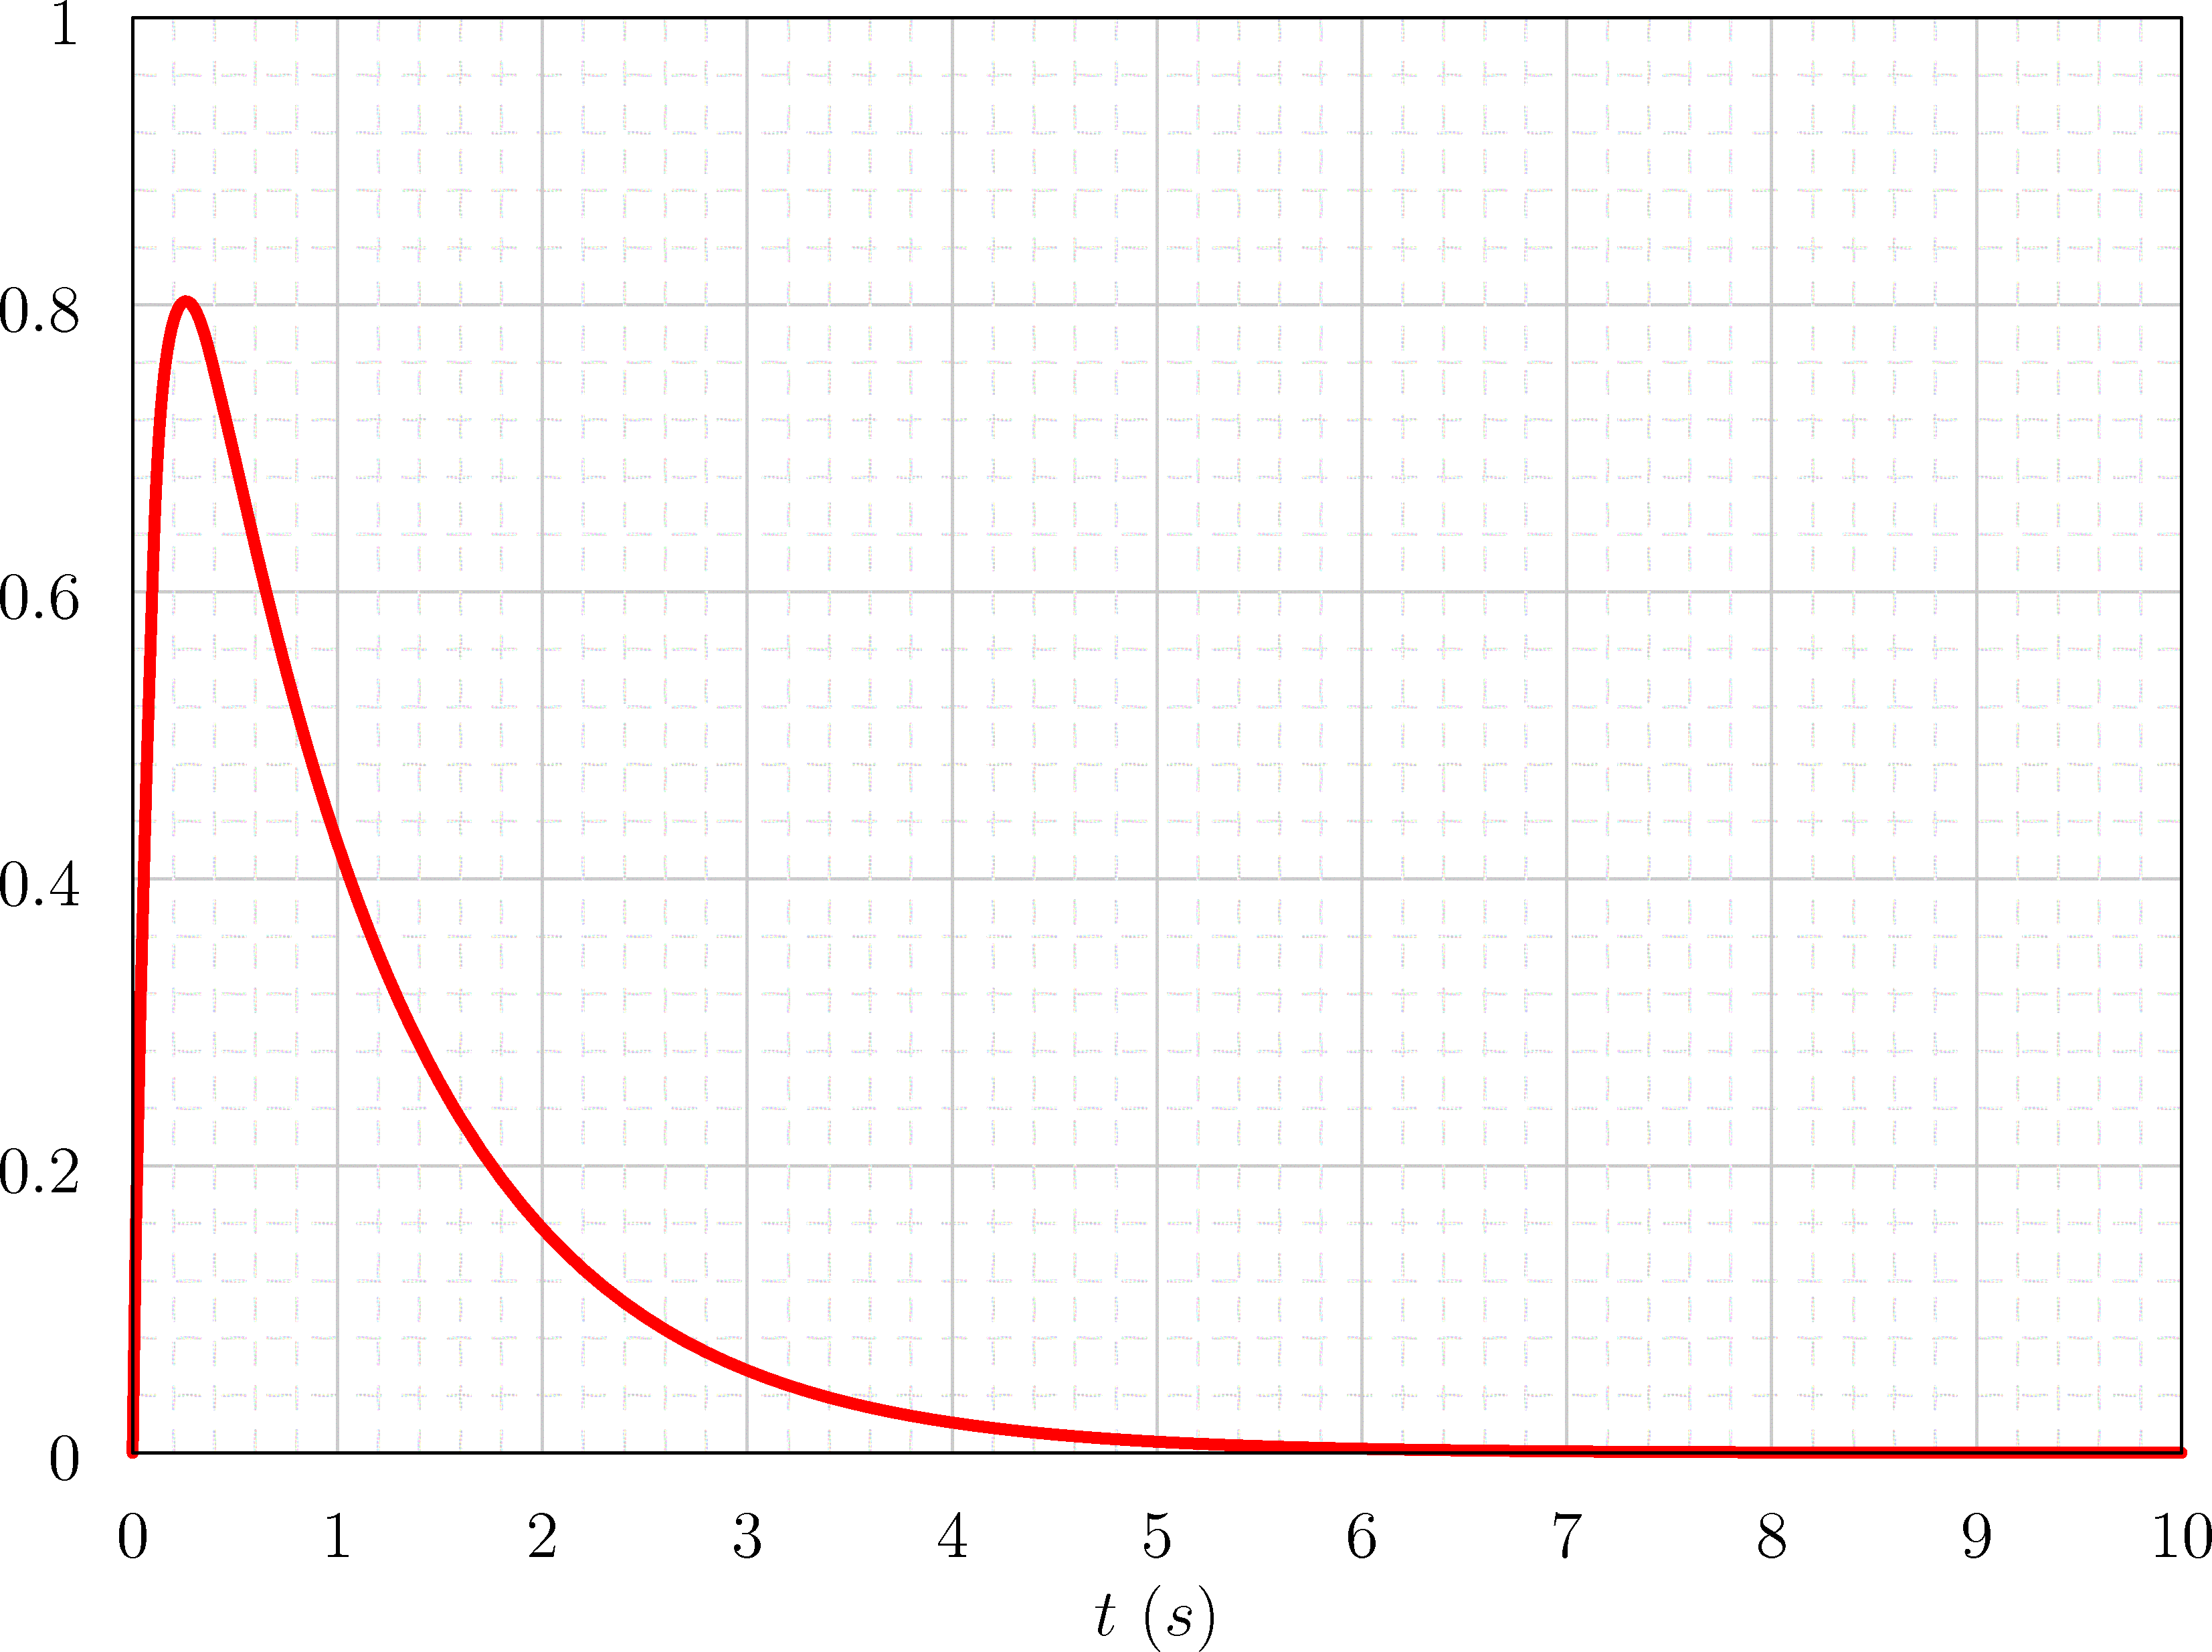
\includegraphics[width=.9\textwidth]{png/ordre2_dirac_1}

\textit{Réponse impulsionnelle d'un système \\ du second ordre -- Cas où $\xi > 1$}
\end{center}
\end{minipage}

\subsection{Cas 2 : $\xi<1$}

\begin{minipage}[c]{.46\linewidth}
Dans le domaine temporel, on a :

$$
s(t)=\dfrac{K\omega_0}{\sqrt{1-\xi^2}}e^{-\xi\omega_0t}\sin\left(\omega_0
t\sqrt{1-\xi^2} \right) u(t) 
$$

La pseudo-période des oscillations vaut :
$$
T=\dfrac{2\pi}{\omega_0\sqrt{1-\xi^2}}
$$

Lorsqu'il n'y a pas d'amortissement ($\xi=0$) on a une réponse sinusoïdale de
pulsation $\omega_0$. 

\end{minipage} \hfill
\begin{minipage}[c]{.46\linewidth}
\begin{center}
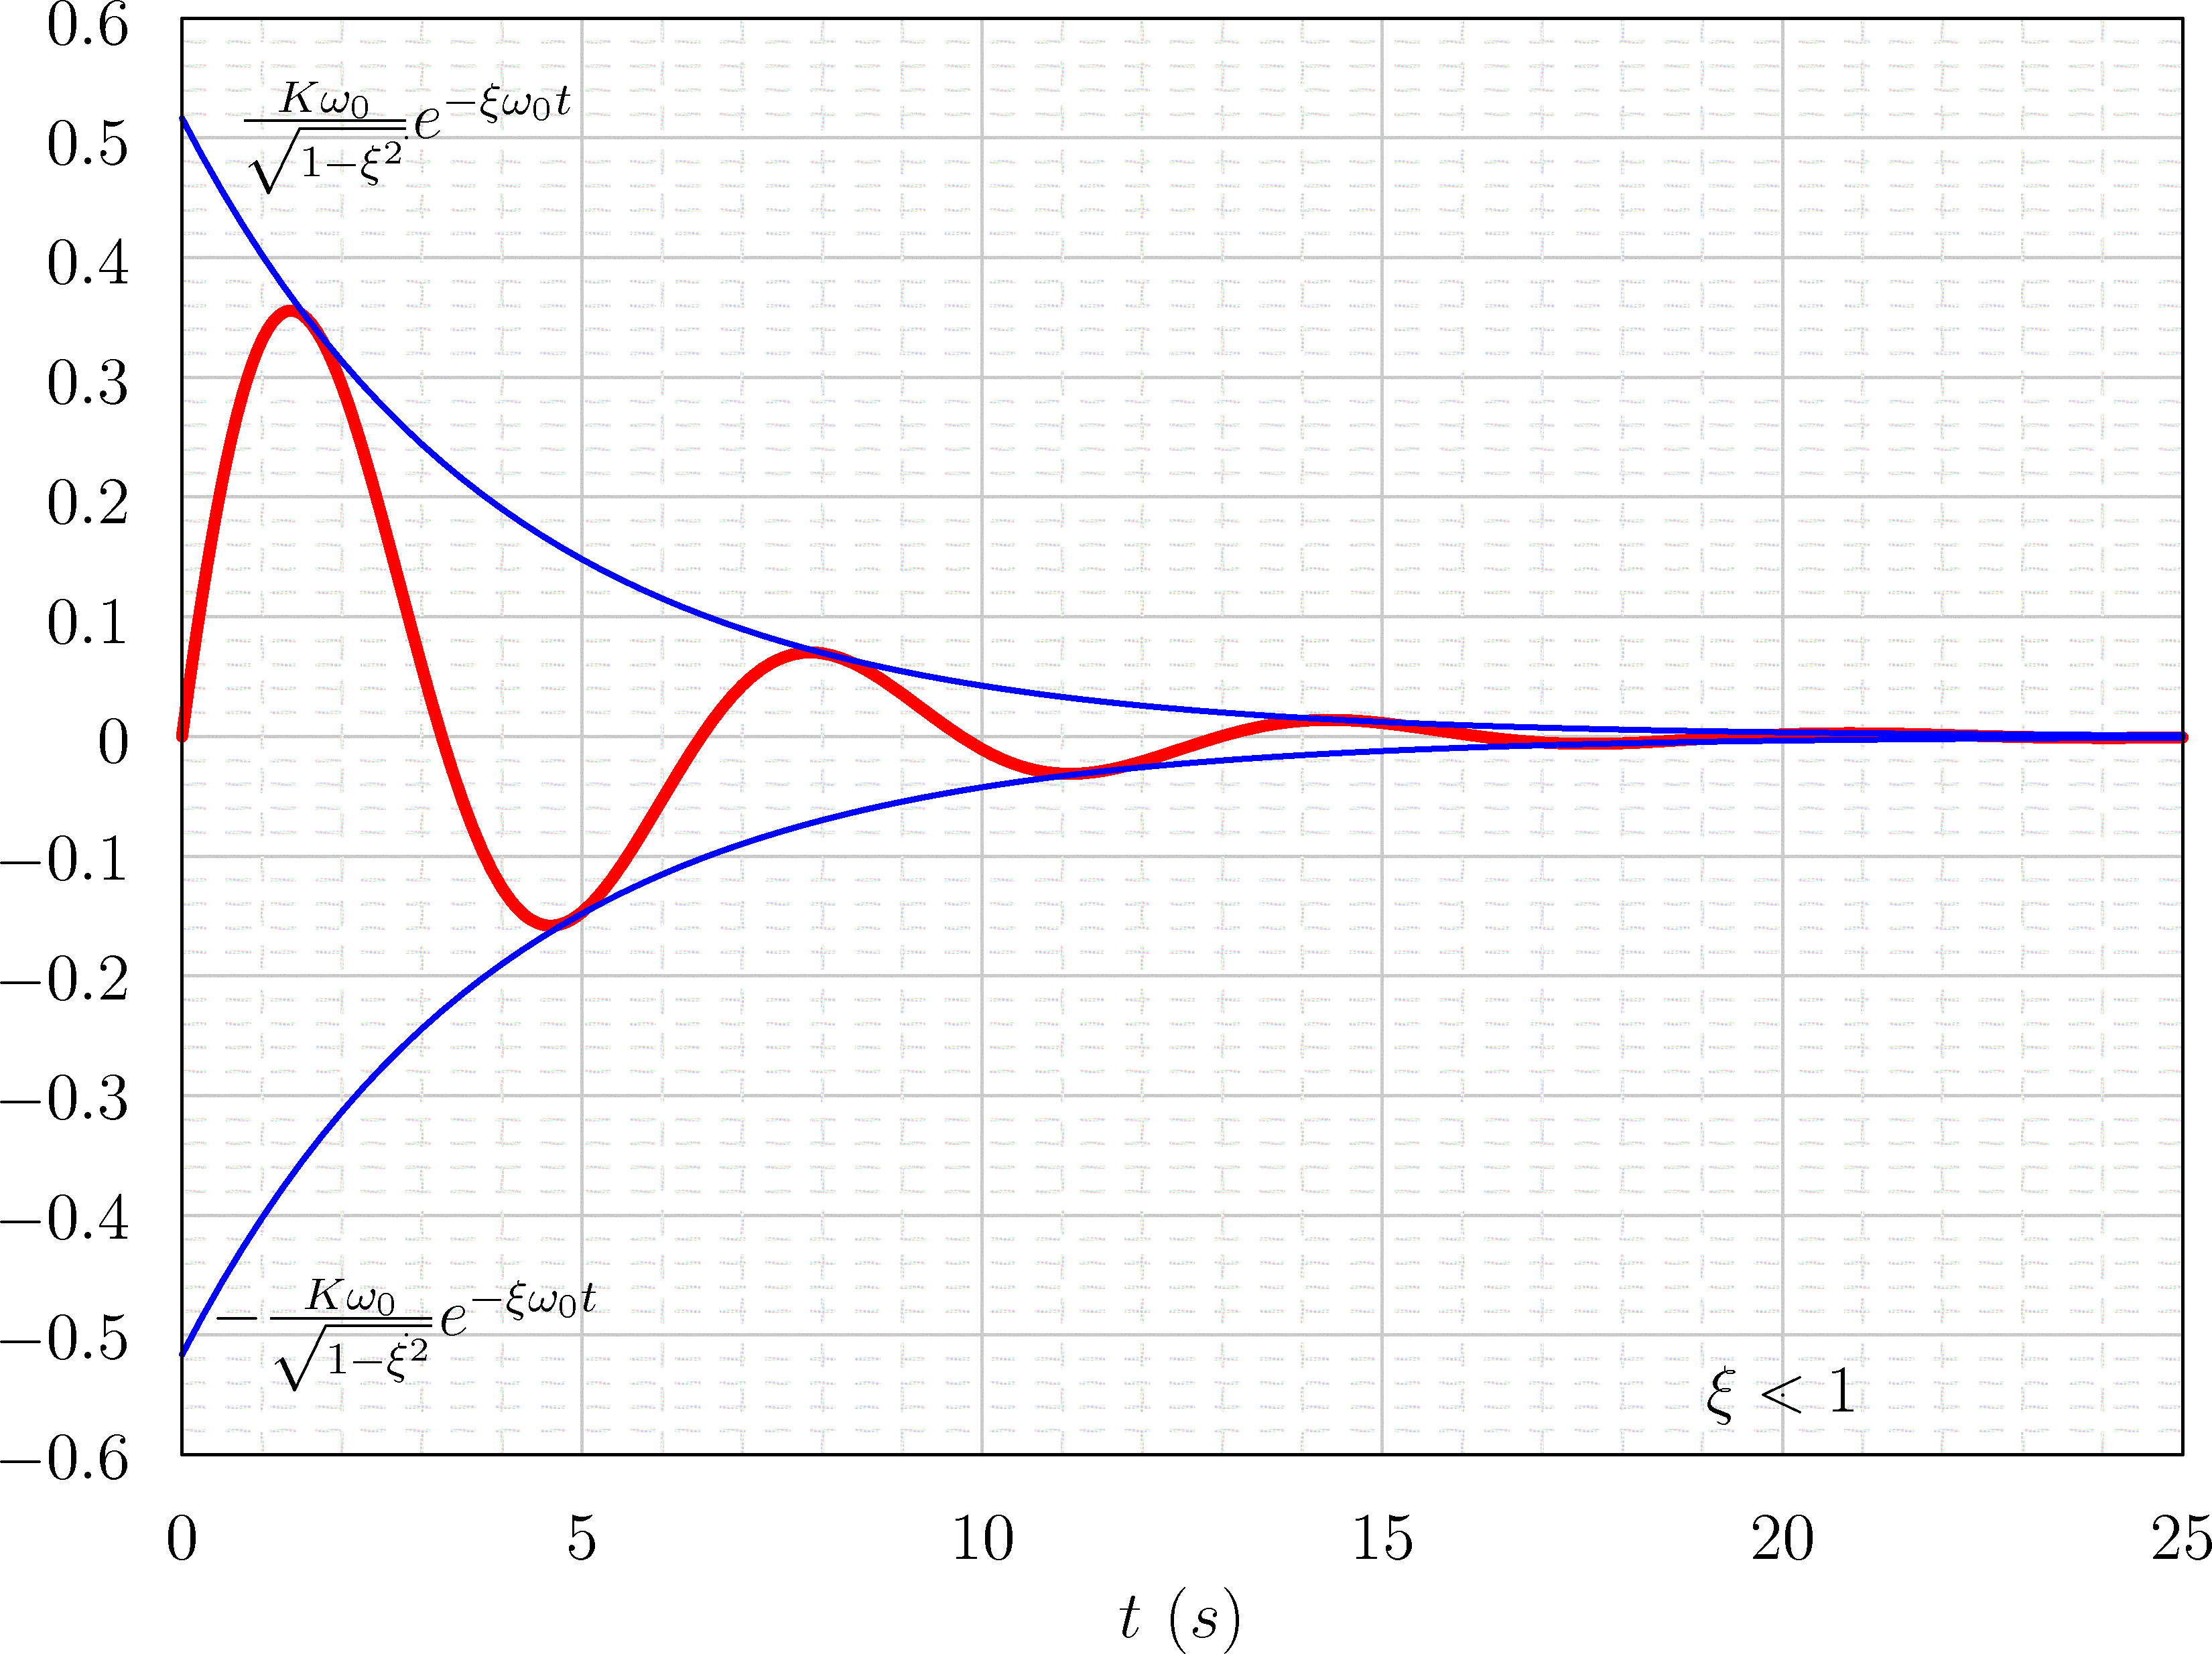
\includegraphics[width=.9\textwidth]{png/ordre2_dirac_c2_1}

\textit{Réponse impulsionnelle d'un système \\ du second ordre -- Cas où $\xi<1$}
\end{center}

\end{minipage}

\subsection{Cas 3 : $\xi=1$}
Dans ce cas $D(p)$ possède une racine double.

L'allure de la réponse serait comparable à celle obtenue dans le cas du régime
apériodique mais ce cas est impossible dans la réalité : on ne peut avoir une
valeur réelle de $\xi$ exactement égale à 1. 


\section{Réponse indicielle}
%\textbf{Remarque :}
%La réponse indicielle est l'intégrale de 0 à $t$ de la réponse impulsionnelle. 
%En effet, $S_{imp}=H(p)\cdot 1$ et $S_{ind}=H(p)\cdot 1=\dfrac{1}{p}$.

%La réponse impulsionnelle étant nulle pour $t=0$, la pente de la réponse
%indicielle est nulle à l'origine. 
Dans ce cas, 
$$
S(p)=\dfrac{1}{p}\cdot H(p)
$$
\subsection{Cas 1 : $\xi > 1$}



Dans ce cas, $D(p)$ possède 2 racines réelles notées $p_1$ et $p_2$ :
$$
\left\{
\begin{array}{l}
p_1 =
\dfrac{-2\xi\omega_0-\sqrt{\Delta}}{2}=-\xi\omega_0-\omega_0\sqrt{\xi^2-1}\\ 
p_2 =
\dfrac{-2\xi\omega_0+\sqrt{\Delta}}{2}=-\xi\omega_0+\omega_0\sqrt{\xi^2-1}\\ 
\end{array}
\right.
$$

On a $p_1<p_2<0$.

En notant $\tau_1=-\dfrac{1}{p_1}$ et $\tau_2=-\dfrac{1}{p_2}$, la fonction de
transfert $H(p)$ peut s'écrire sous la forme suivante :  
$$
H(p)=\dfrac{K}{\left(1+ \tau_1 p \right)\left(1+ \tau_2 p  \right)}
$$

En conséquence, 
$$
S(p)=\dfrac{1}{p}\cdot\dfrac{K}{\left(1+ \tau_1 p \right)\left(1+ \tau_2 p 
\right)} 
$$

\begin{minipage}[c]{.46\linewidth}

En calculant alors la transformée de Laplace inverse, on obtient :
$$
s(t)=K\left(
1-\dfrac{1}{\tau_1-\tau_2}\cdot\left(
\tau_1e^{-t\dfrac{t}{\tau_1}}-\tau_2e^{-t\dfrac{t}{\tau_2}}
\right)
\right)
$$

On peut aussi mettre $s(t)$ sous la forme suivante : 
$$
s(t)=K\left(
1-\dfrac{1}{2\sqrt{\xi^2-1}}\cdot
\left(\dfrac{e^{p_1t}}{p_1} - \dfrac{e^{p_2t}}{p_2}
\right)\right)
$$

\end{minipage}\hfill
\begin{minipage}[c]{.46\linewidth}

\begin{center}
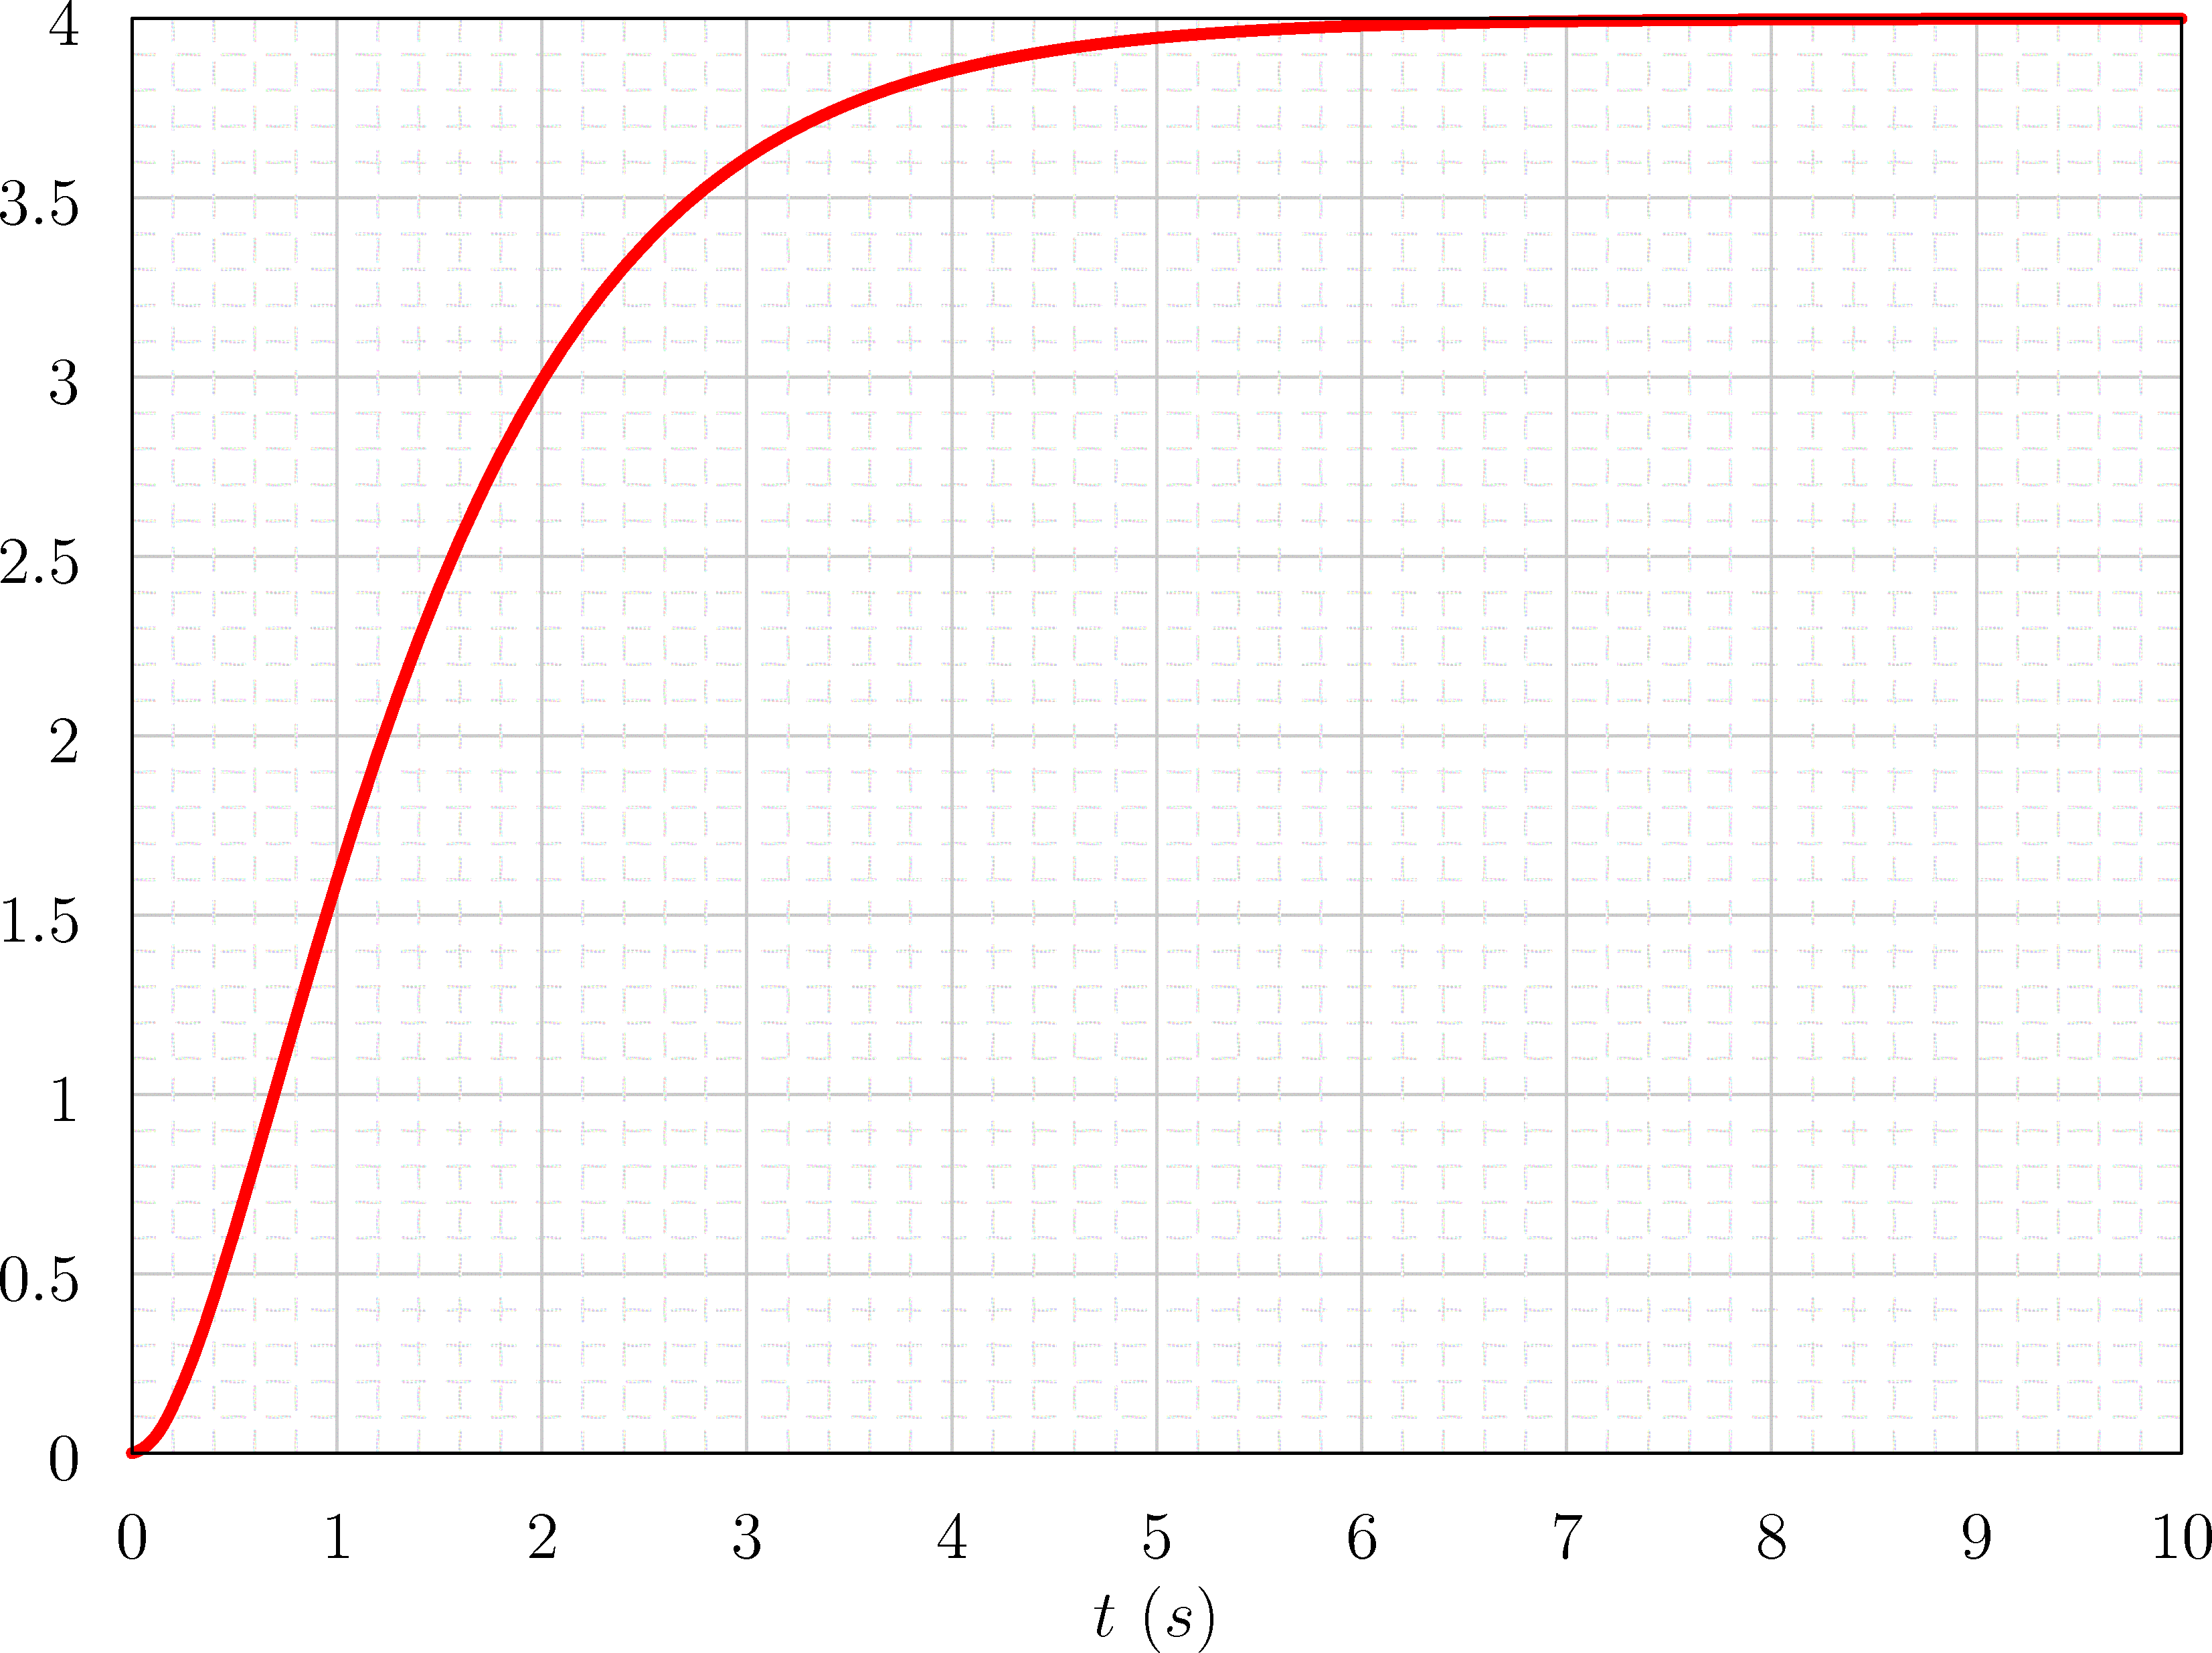
\includegraphics[width=.9\textwidth]{png/ordre2_echelon_c1-1}

\textit{Réponse indicielle d'un système \\ du second ordre -- Cas où $\xi>1$}
\end{center}
\end{minipage}


En $t=0$, la courbe admet une \textbf{tangente horizontale}.

La courbe ne dépasse pas son asymptote horizontale ($s(t)$ est monotone). 

Il n'y a pas de formule pour déterminer le temps de réponse à 5\%.

Nous pouvons remarquer cependant que le système ressemble à un système du
premier ordre lorsqu'on s'éloigne de $t=0$.  

Le temps de réponse à 5\% peut donc être approché par la valeur
$tr_{5\%}=3\times2\xi\omega_0$. 

 %En pratique on utilisera l'abaque des temps de réponse réduits.

\subsection{Cas 2 : $\xi = 1$}

Dans ce cas, $\tau_1=\tau_2=\tau_0$, on parle
d'amortissement critique, l'existence d'un pôle double modifie le décomposition
en éléments simples et on obtient : 

$$
s(t)=K\left(1-\left(1+\dfrac{1}{\tau_0}\right)e^{-\dfrac{t}{\tau_0}}\right)
$$

La réponse est plus rapide que si $\xi>1$ ($tr_{5\%}=5\omega_0$), mais l'allure
de la courbe est très similaire. 

\subsection{Cas 3 : $\xi<1$}
\begin{minipage}[c]{.46\linewidth}
Dans ce cas on parle de système sous amorti.

Dans ce cas, $H(p)$ admet deux pôles complexes conjuguées :
$$
p=-\left( \xi \pm j\sqrt{1-\xi^2}\right)\omega_0
$$

La décomposition de $S(p)$ en éléments simples et le calcul de la transformée de
Laplace inverse nous donne : 
$$
s(t)=K\left[ 1 -
\dfrac{e^{-\xi\omega_0t}}{\sqrt{1-\xi^2}}\cdot\sin\left(\omega_0\sqrt{1-\xi^2}
t+\arccos{\xi}\right)\right] 
$$

\end{minipage}\hfill
\begin{minipage}[c]{.46\linewidth}

\begin{center}
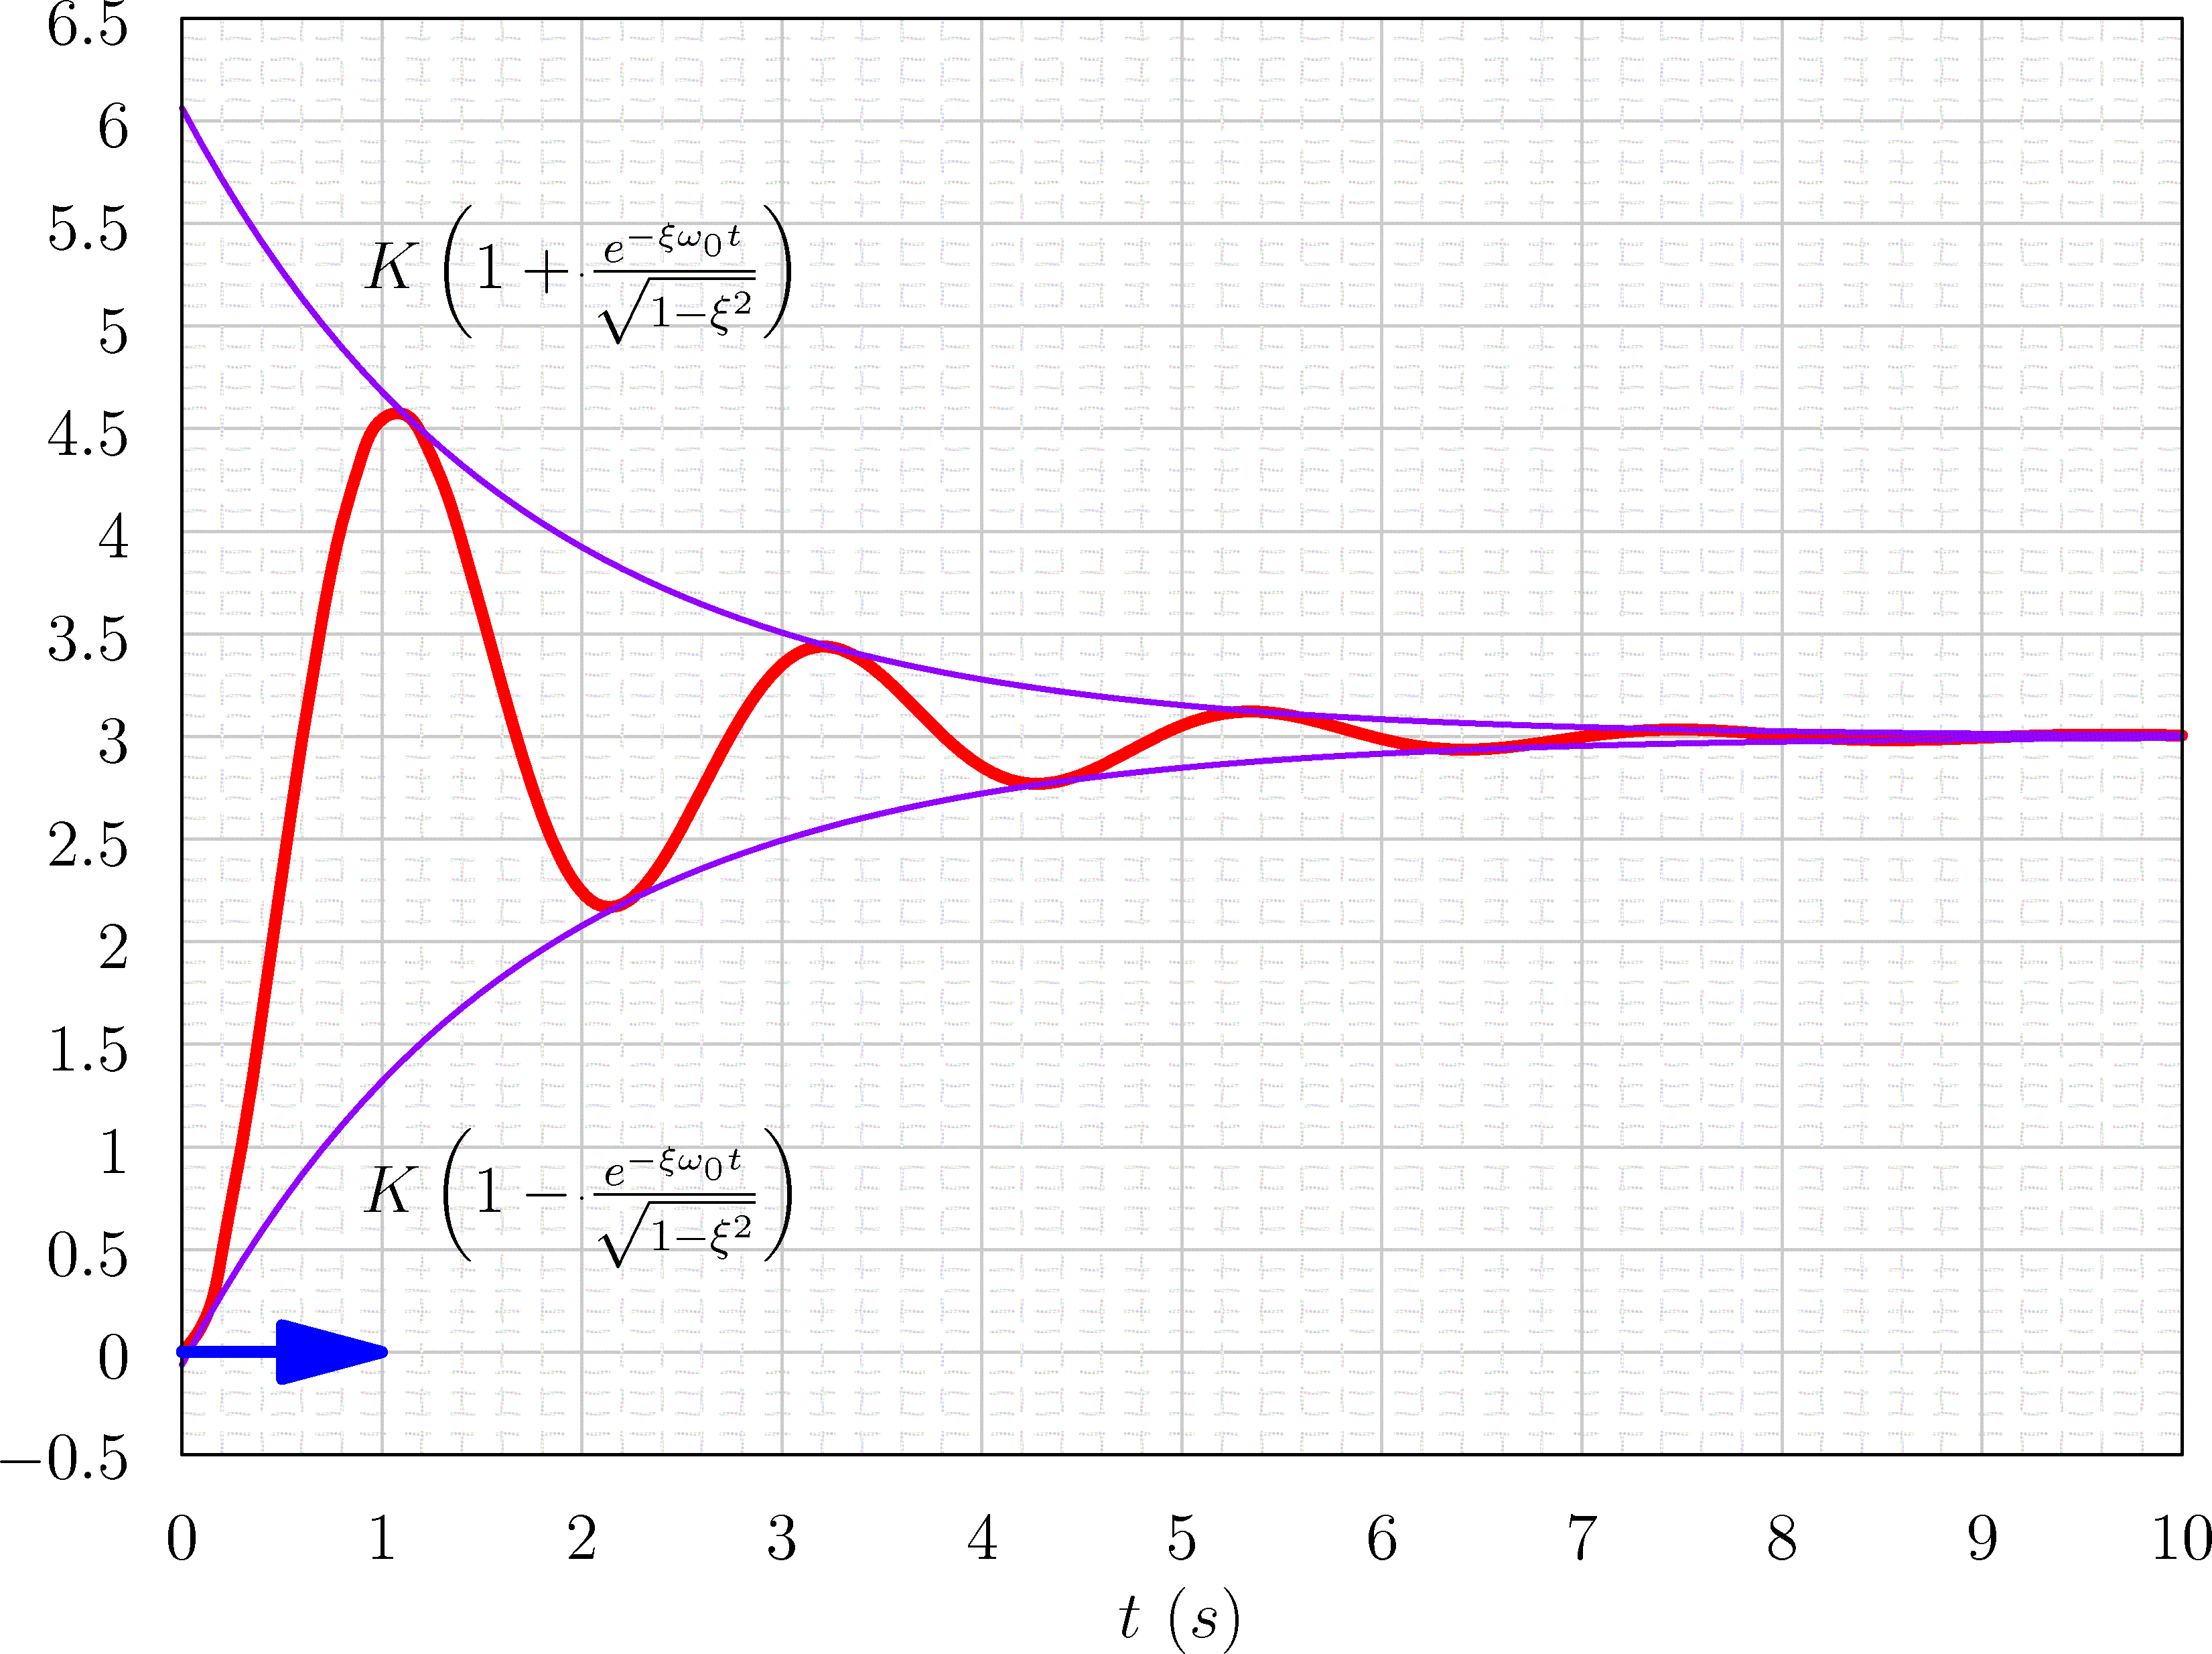
\includegraphics[width=.9\textwidth]{png/ordre2_echelon_c2}
\end{center}
\end{minipage}

La courbe admet toujours une tangente horizontale à $t=0$.

On observe l'apparition d'oscillations autour de la valeur finale (réponse
pseudo-périodique), d'autant plus amorties que $\xi$ est élevé. Pour $\xi=0$, la
réponse est sinusoïdale d'amplitude $2K$.  

Les courbes enveloppes ont pour équation les courbes suivantes : 
$$
y(t)=K\left( 
1\pm \dfrac{e^{-\xi\omega_0 t}}{\sqrt{1-\xi^2}}
\right)
$$

\begin{rem}
On définit parfois $\omega_p$ :
$$
\omega_p = \omega_0 \sqrt{1-\xi^2}
$$
\end{rem}

\begin{resultat}
La pseudo-période des oscillations est donnée par :

$$
T_p=\dfrac{2\pi}{\omega_0\sqrt{1-\xi^2}}
$$

\end{resultat}

\subsubsection{Résultats sur les dépassements}

\begin{minipage}[c]{.4\linewidth}
Lorsque $\xi$ est inférieur à 1, la réponse indicielle génère des dépassements. 


\begin{resultat}
On montre que le premier dépassement est obtenu pour :
\ifthenelse{\boolean{prof}}{%
$$
t_1 = \dfrac{\pi}{\omega_0\sqrt{1-\xi^2}}=\dfrac{T_p}{2}
$$
}{
\rotatebox{90}{
\begin{tabular}{p{1.5cm}}
\\
\end{tabular}}
}

\end{resultat}

\end{minipage}\hfill
\begin{minipage}[c]{.55\linewidth}
\begin{center}
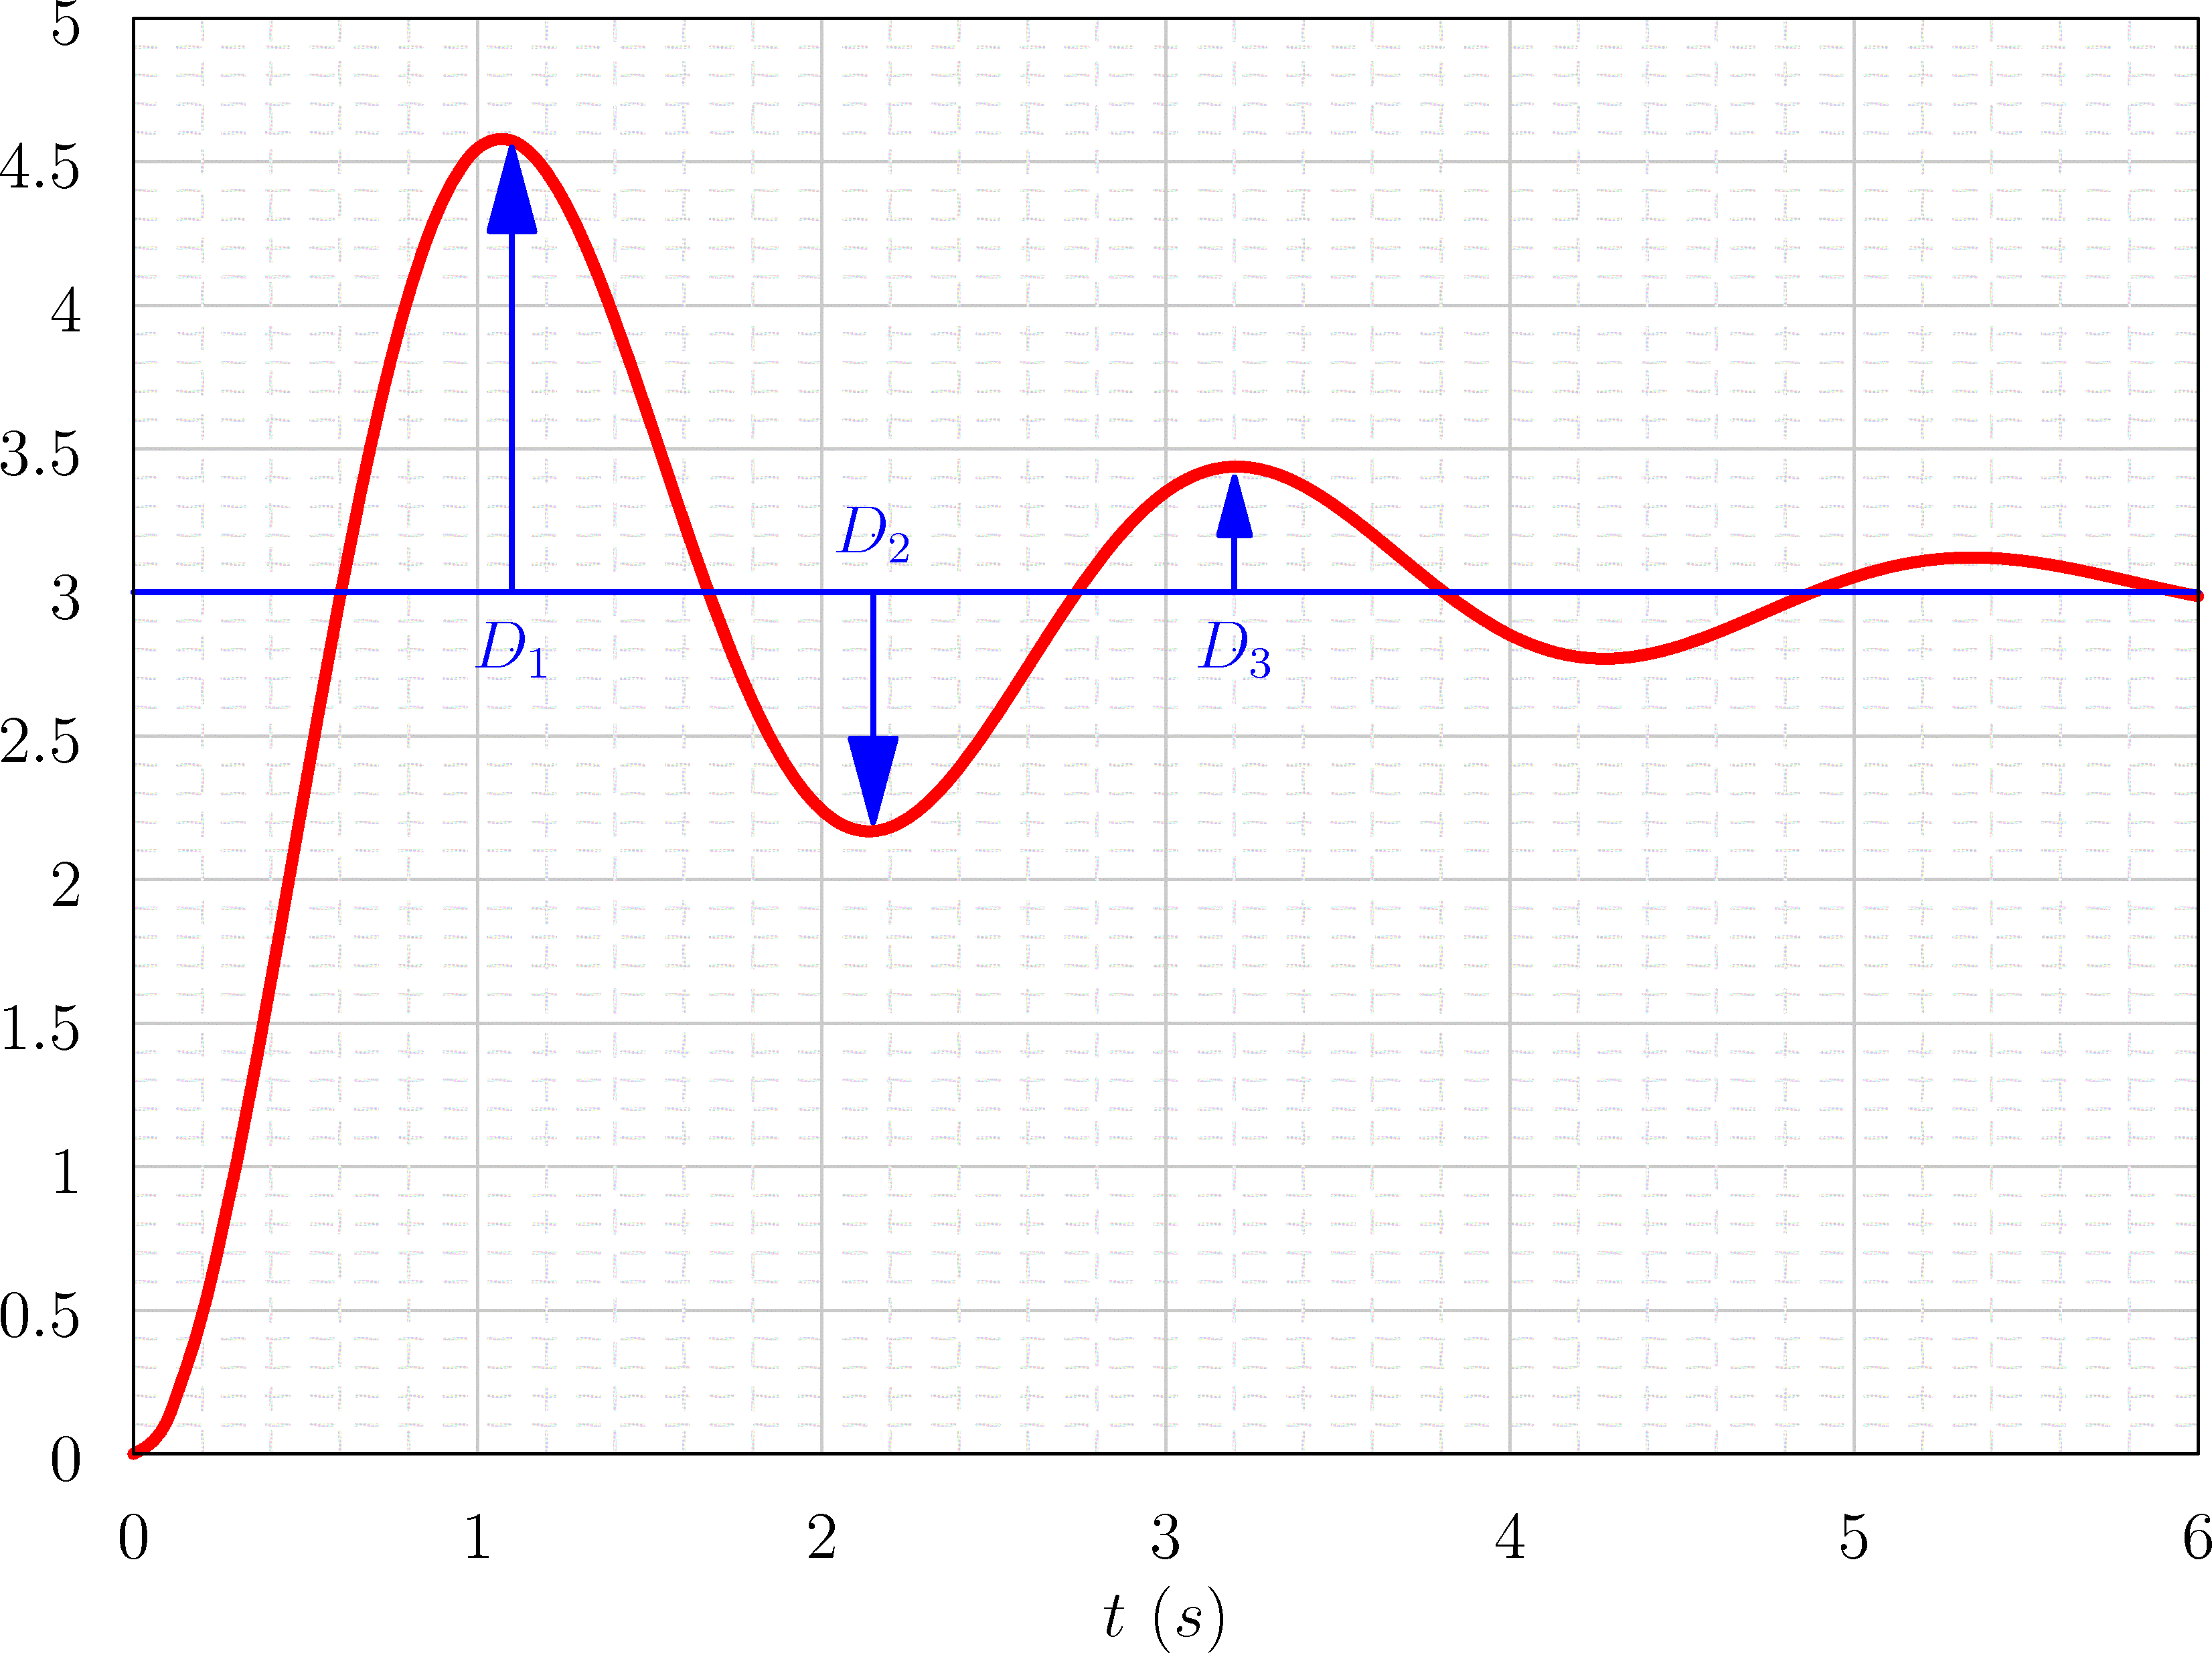
\includegraphics[width=.9\textwidth]{png/depassement2}
\end{center}
\end{minipage}


La valeur du dépassement (en pourcentage) peut se calculer alors ainsi :

$$
D_{1\%} = \left| \dfrac{s(t_1)-s(\infty)}{s(\infty)-s(0)}\right|
$$

\begin{resultat}
Le premier dépassement pour cent vaut : 

\vfill

\ifthenelse{\boolean{prof}}=e^{\dfrac{-\pi \xi}{\sqrt{1-\xi^2}}}
$$
}{
\rotatebox{90}{
\begin{tabular}{p{1.5cm}}
\\
\end{tabular}}}

\vfill

La valeur du pic est donnée par $D_{1\%}\cdot K \cdot E_0$ ($E_0$ valeur de l'échelon d'entrée).

\end{resultat}

\begin{resultat}
Le k\ieme dépassement pour cent vaut : 

\ifthenelse{\boolean{prof}}=e^{\dfrac{-k \pi \xi}{\sqrt{1-\xi^2}}}
$$
}{
\rotatebox{90}{
\begin{tabular}{p{1.5cm}}
\\
\end{tabular}}}
\end{resultat}

L'abaque ci-dessous permet de connaître la valeur du k\ieme  dépassement \textbf{pour cent} en fonction du facteur d'amortissement. 
Lorsque l'amortissement tend vers 1, on peut ainsi mettre en évidence que la valeur des dépassements est de plus en plus faible.

\begin{center}
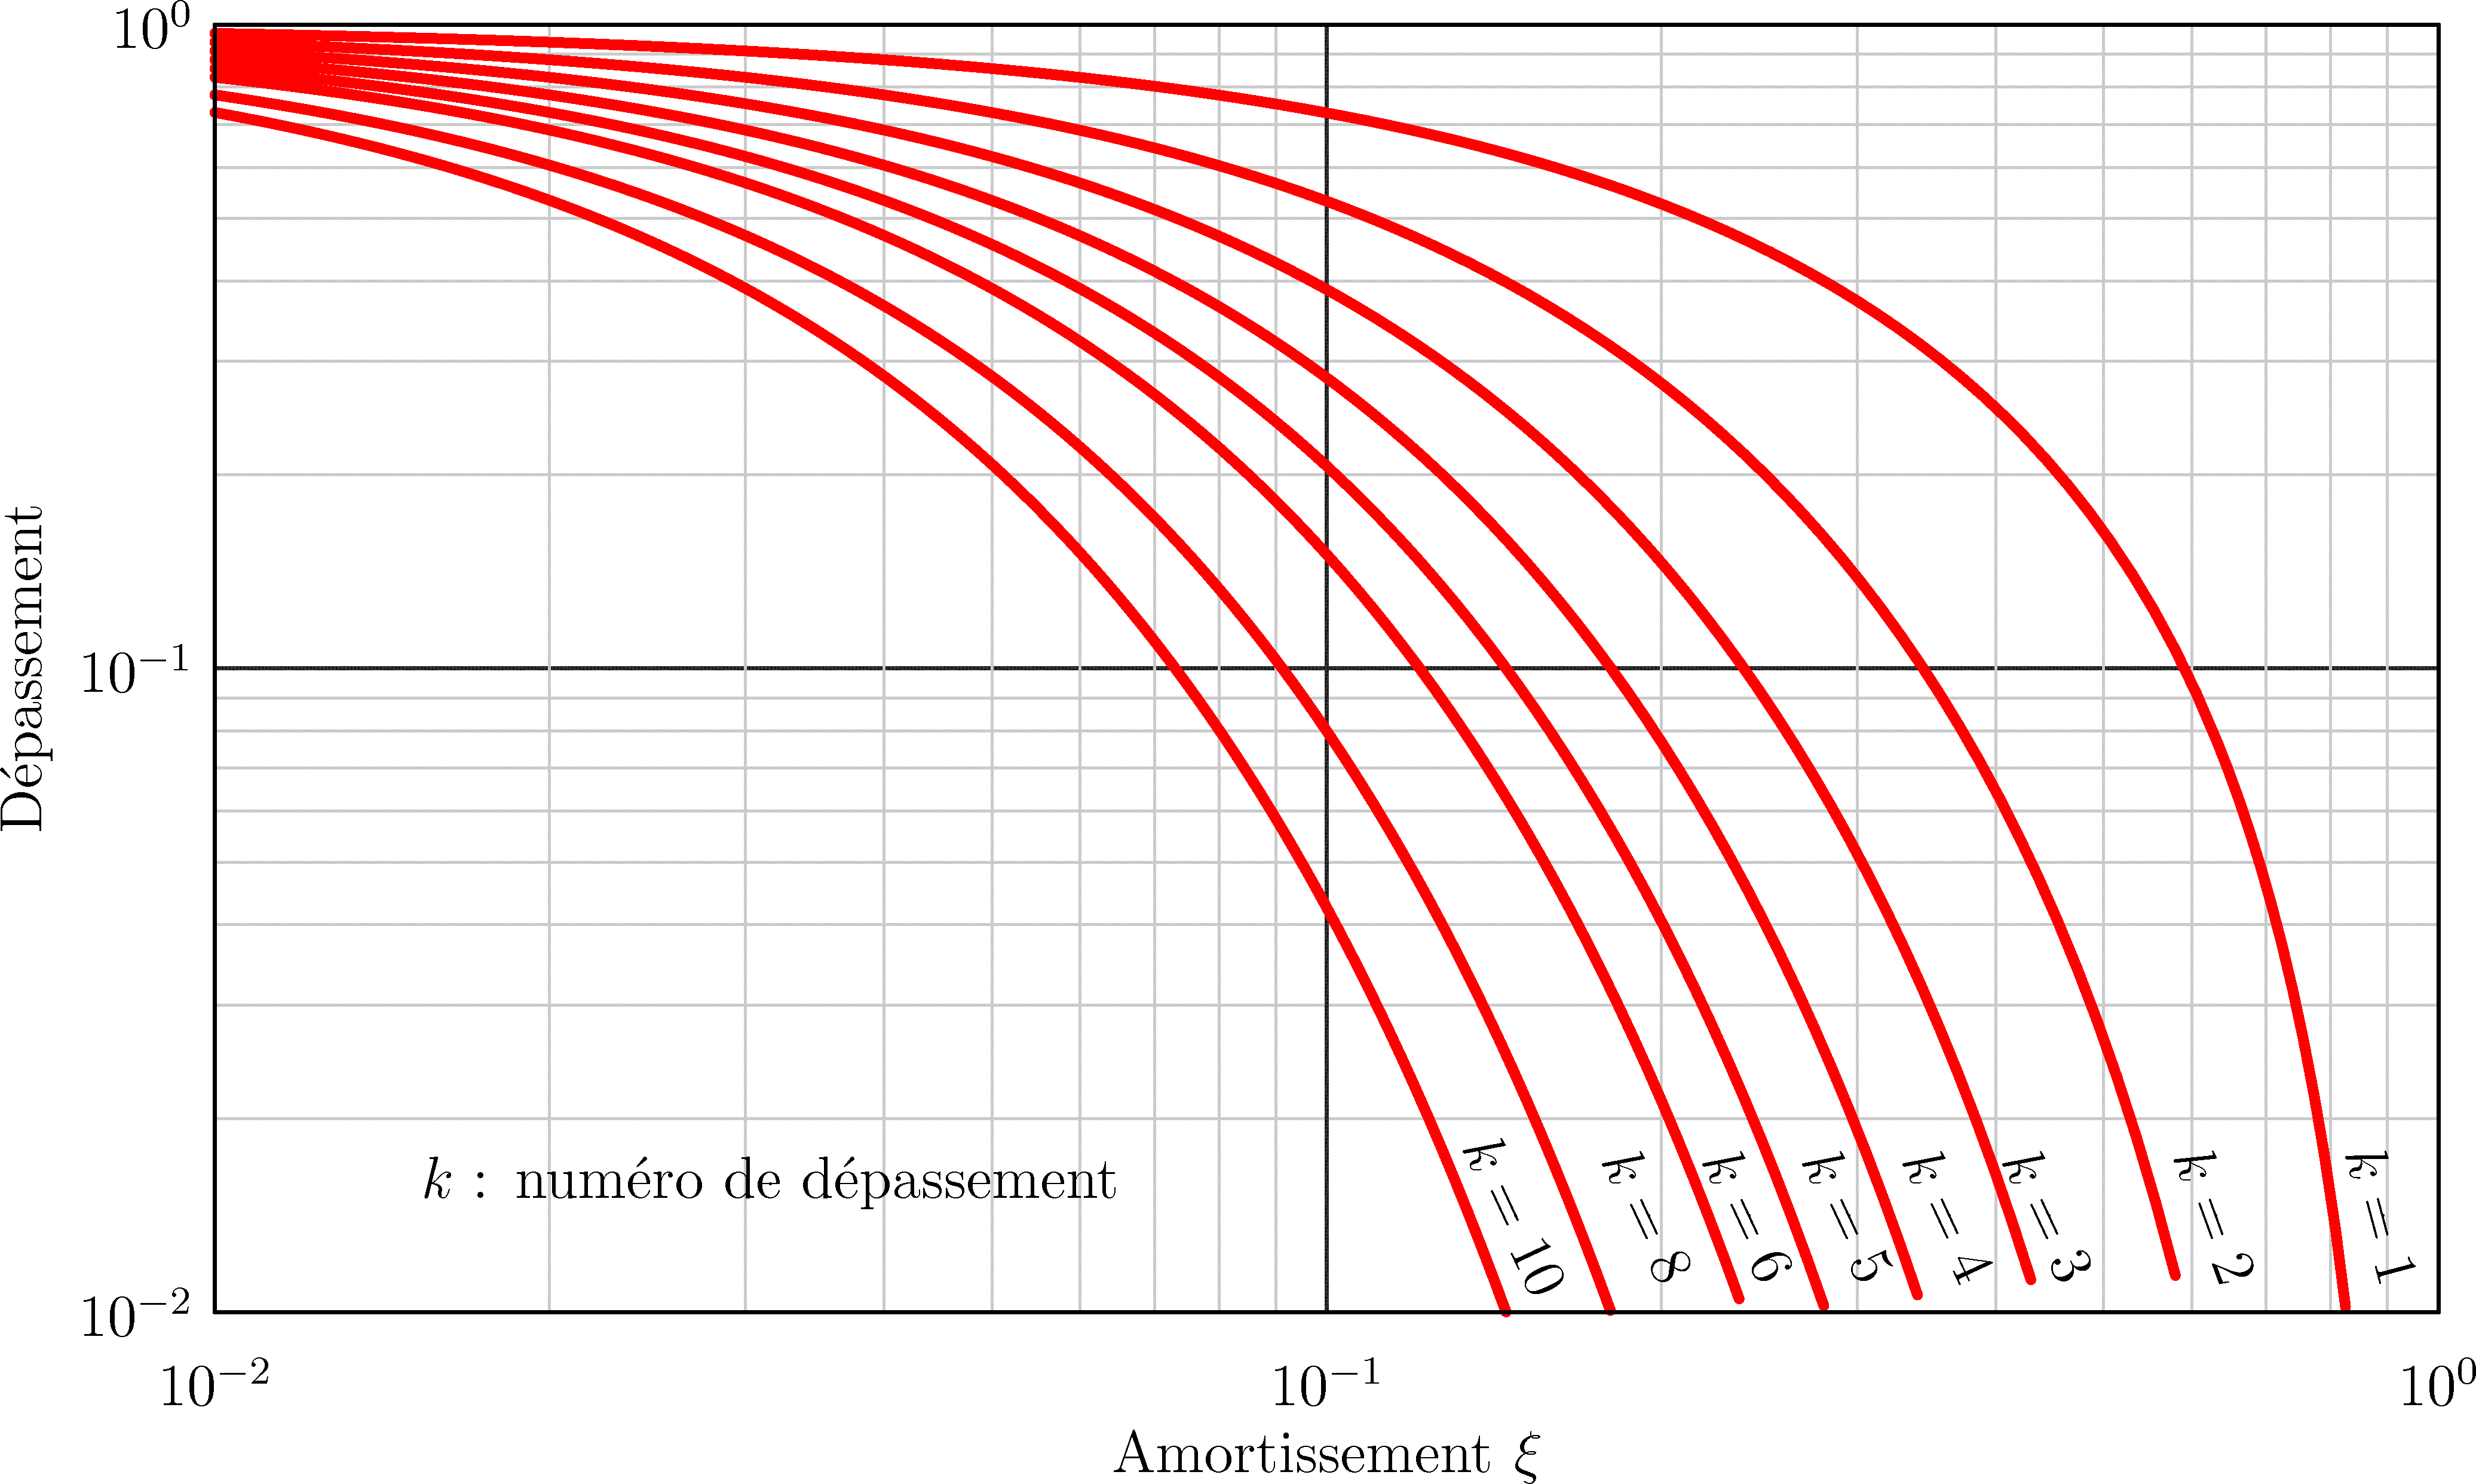
\includegraphics[width=.7\textwidth]{png/depassement}
\end{center}




\subsubsection{Résultat sur le temps de réponse à 5\%}
\begin{minipage}[c]{.4\linewidth}
La rapidité d'un système du second ordre va se calculer par le temps de réponse à 5\%. Le temps de réponse dépend de $\omega_0$ et $\xi$ et ne pas s'écrire sous une forme analytique simple. 

L'abaque ci-contre donne le temps de réponse réduit $tr_{5\%} \omega_0$ en fonction du coefficient d'amortissement $\xi$. 
\begin{resultat}
On note que le temps de réponse est minimum lorsque $\xi\simeq 0,7$. Dans ces conditions :
$$
t_{r5\%} \cdot \omega_0 = 3
$$
\end{resultat}
\end{minipage}\hfill
\begin{minipage}[c]{.55\linewidth}
\begin{center}
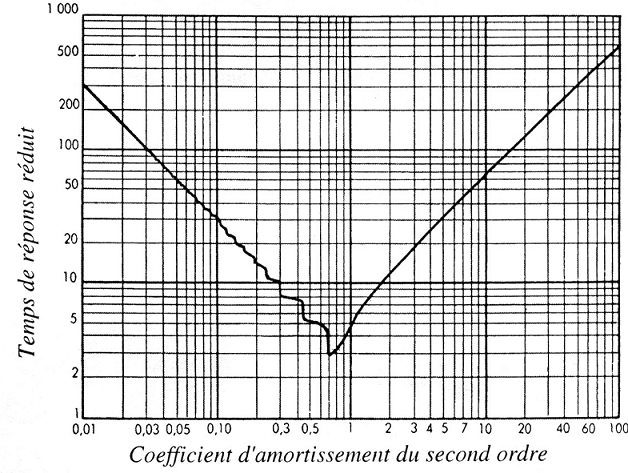
\includegraphics[width=.95\textwidth]{png/tr}
\end{center}
\end{minipage}


\subsection{Évolution de la réponse en fonction du coefficient d'amortissement}


\begin{center}
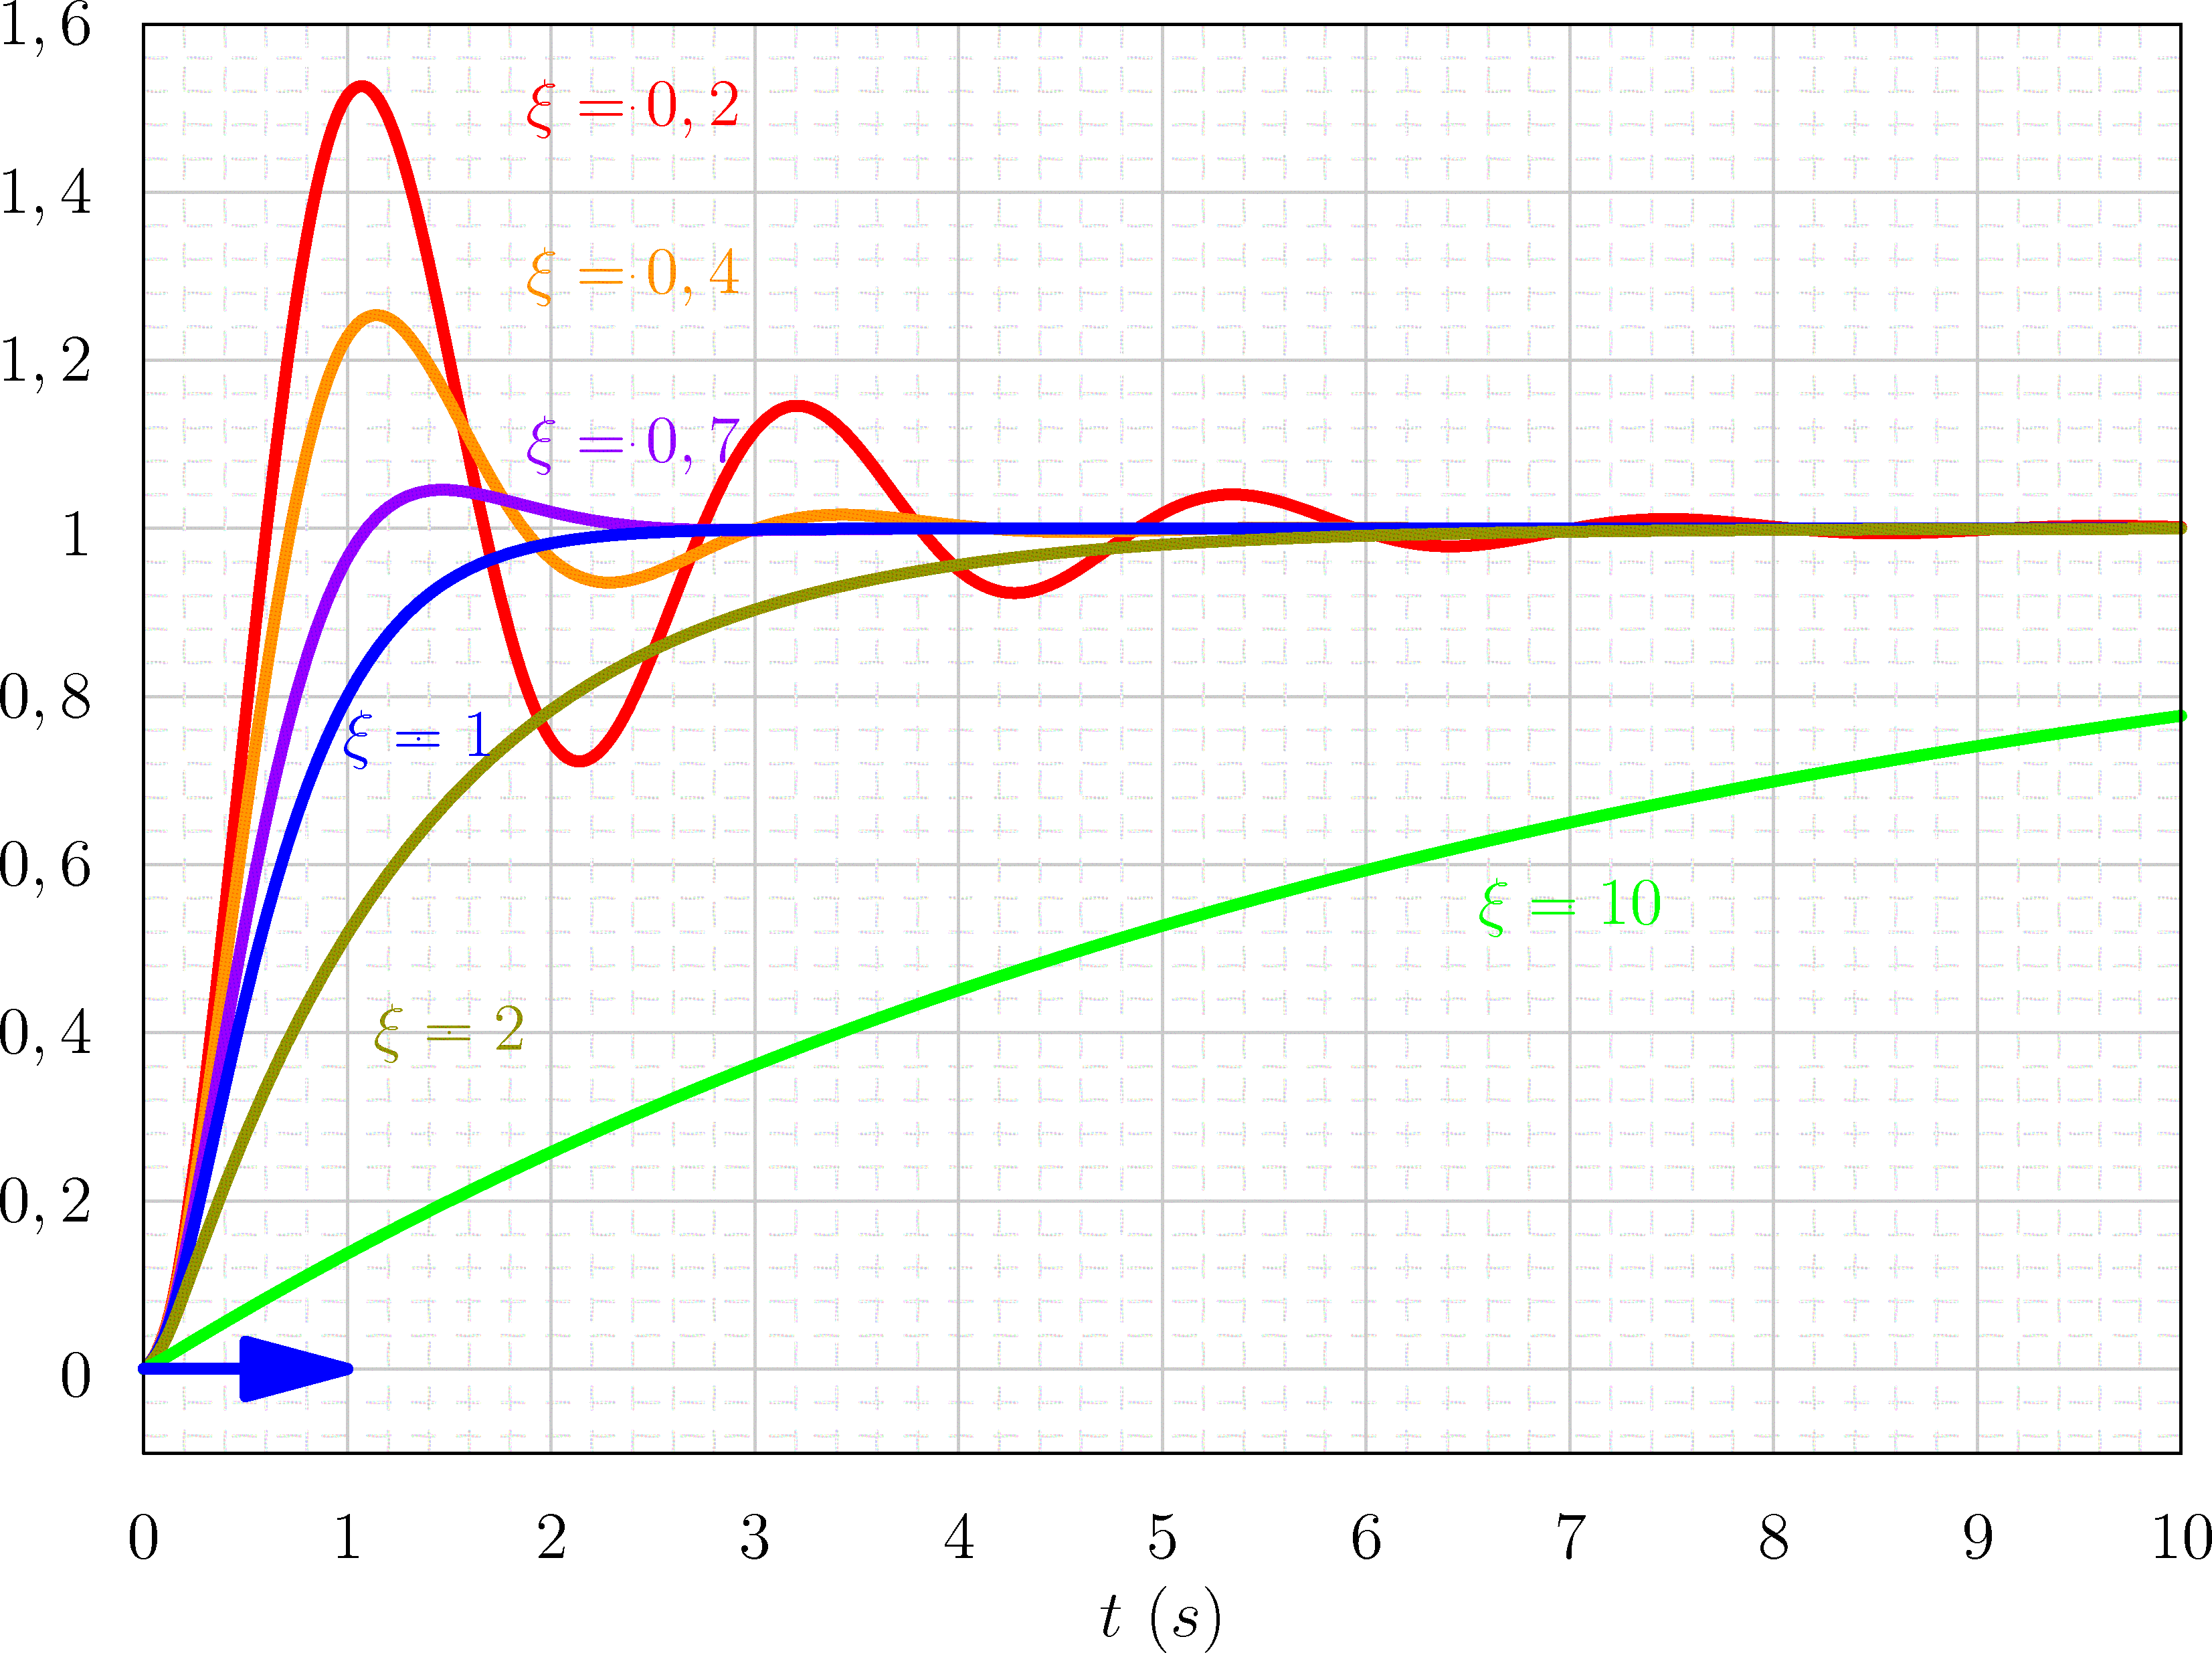
\includegraphics[width=.7\textwidth]{png/ordre2_echelon_z}
\end{center}


\begin{resultat}
On peut montrer que pour la réponse indicielle d'un système du second ordre 
\begin{itemize}
\item il existe une tangente horizontale à l'origine;
\item la valeur finale tend vers $K E_0$ (si l'échelon d'entrée vaut $E_0$).
\end{itemize}
\end{resultat}
\end{document}

\newpage

%\section{Annexes}
\subsection{Calcul de la réponse impulsionnelle}

\subsubsection{Cas 1 : $\xi>1$}

Dans ce cas, $D(p)$ possède 2 racines réelles notées $p_1$ et $p_2$ :
%$$
%\left\{
%\begin{array}{l}
%p_1 =
%\dfrac{-2\xi\omega_0-\sqrt{\Delta}}{2}=\xi\omega_0-\omega_0\sqrt{\xi^2-1}\\ 
%p_2 =
%\dfrac{-2\xi\omega_0+\sqrt{\Delta}}{2}=\xi\omega_0+\omega_0\sqrt{\xi^2-1}\\ 
%\end{array}
%\right.
%$$

$$
p_{1,2} 
=
\dfrac{-\dfrac{2\xi}{\omega_0}\pm\sqrt{\Delta}}{\dfrac{2}{\omega_0^2}}
=\dfrac{-2\xi\omega_0\pm\omega_0^2\sqrt{\Delta}}{2}
=-\xi\omega_0\pm\omega_0\sqrt{ \xi^2 -1}
$$


On peut donc écrire $S(p)$ sous la forme suivante : 
$$
S(p)=\dfrac{K}{\dfrac{1}{\omega_0^2}\left(p-p_1\right)\left(p-p_2\right)}
$$

%\end{minipage}\hfill
%\begin{minipage}[c]{.46\linewidth}

La décomposition en éléments simples de $S(p)$ donne : 
$$
S(p)
%=K\omega_0^2\left( \dfrac{\alpha}{p-p_1} + \dfrac{\beta}{p-p_2} \right) 
=\dfrac{K\omega_0^2}{2\omega_0\sqrt{\xi^2-1}}\left( \dfrac{1}{p-p_1} - \dfrac{1}{p-p_2} \right) 
%\dfrac{K\omega_0}{2\sqrt{\xi^2-1}}\left( \dfrac{1}{p-p_1} - \dfrac{1}{p-p_2}
%\right) 
$$

D'après la transformée de Laplace inverse, on a : 
$$
s(t)=\dfrac{K\omega_0}{2\sqrt{\xi^2-1}} \left(e^{p_1 t}-e^{p_2 t} \right)\cdot
u(t) 
$$



\subsubsection{Cas 2 : $\xi<1$}


Dans ce cas, $S(p)$ s'écrit sous la forme :
$$
S(p)=\dfrac{K\omega_0^2}{\left(p+\xi\omega_0 \right)^2+\omega_0^2\left(1-\xi^2
\right)} 
$$

On note : 
\begin{itemize}
\item $\omega^2 = \omega_0^2 \left(1-\xi^2 \right)$
\item $a=\xi\omega_0$
\end{itemize}

En conséquence : 
$$
S(p)=\dfrac{K\omega_0}{\sqrt{1-\xi^2}}
\dfrac{\omega}{\left(p+a\right)^2+\omega^2} 
$$

En repassant dans le domaine temporel, on a :

$$
s(t)=\dfrac{K\omega_0}{\sqrt{1-\xi^2}}e^{-\xi\omega_0t}\sin\left(\omega_0
t\sqrt{1-\xi^2} \right) u(t) 
$$

\subsection{Calcul de la réponse indicielle}

\subsubsection{Cas 1 : $\xi\geq1$}
%\subsubsection{Réponse temporelle}
Dans ce cas, $D(p)$ possède 2 racines réelles notées $p_1$ et $p_2$ :
$$
\left\{
\begin{array}{l}
p_1 =
\dfrac{-2\xi\omega_0-\sqrt{\Delta}}{2}=\xi\omega_0-\omega_0\sqrt{\xi^2-1}\\ 
p_2 =
\dfrac{-2\xi\omega_0+\sqrt{\Delta}}{2}=\xi\omega_0+\omega_0\sqrt{\xi^2-1}\\ 
\end{array}
\right.
$$

On a $p_1<p_2<0$.

En notant $\tau_1=-\dfrac{1}{p_1}$ et $\tau_2=-\dfrac{1}{p_2}$, la fonction de
transfert $H(p)$ peut s'écrire sous la forme suivante :  
$$
H(p)=\dfrac{K}{\left(1+ \tau_1 p \right)\left(1+ \tau_2 p  \right)}
$$

En conséquence, 
$$
S(p)=\dfrac{1}{p}\cdot\dfrac{K}{\left(1+ \tau_1 p \right)\left(1+ \tau_2 p 
\right)} 
$$
En décomposant $S(p)$ en éléments simples et en calculant $\alpha$, $\beta$ et
$\gamma$ on obtient : 

$$
S(p)=K\left[
\dfrac{1}{p}-\dfrac{\tau_1^2}{\tau_1-\tau_2}\cdot\dfrac{1}{1+\tau_1 p} -
\dfrac{\tau_2^2}{\tau_1-\tau_2}\cdot\dfrac{1}{1+\tau_2 p} 
\right]
$$


En calculant alors la transformée de Laplace inverse, on obtient :
$$
s(t)=K\left(
1-\dfrac{1}{\tau_1-\tau_2}\cdot\left(
\tau_1e^{-t\dfrac{t}{\tau_1}}-\tau_2e^{-t\dfrac{t}{\tau_2}}
\right)
\right)
$$

On peut aussi mettre $s(t)$ sous la forme suivante : 
$$
s(t)=K\left(
1-\dfrac{1}{2\sqrt{\xi^2-1}}\cdot
\left(\dfrac{e^{p_1t}}{p_1} - \dfrac{e^{p_2t}}{p_2}
\right)\right)
$$


\subsubsection{Cas 2 : $\xi<1$}
Dans ce cas on parle de système sous amorti.

Dans ce cas, $H(p)$ admet deux pôles complexes conjuguées :
$$
p=-\left( \xi \pm j\sqrt{1-\xi^2}\right)\omega_0
$$

La décomposition de $S(p)$ en éléments simples et le calcul de la transformée de
Laplace inverse nous donne : 
$$
s(t)=K\left[ 1 -
\dfrac{e^{-\xi\omega_0t}}{\sqrt{1-\xi^2}}\cdot\sin\left(\omega_0\sqrt{1-\xi^2}
t+\arccos{\xi}\right)\right] 
$$



La courbe admet toujours une tangente horizontale à $t=0$.

On observe l'apparition d'oscillations autour de la valeur finale (réponse
pseudo-périodique), d'autant plus amorties que $\xi$ est élevé. Pour $\xi=0$, la
réponse est sinusoïdale d'amplitude $2K$.  

La pseudo-période des oscillations est donnée par :
$$
T=\dfrac{2\pi}{\omega_0\sqrt{1-\xi^2}}
$$

Les courbes enveloppes ont pour équation les courbes suivantes : 
$$
y(t)=K\left( 
1\pm \dfrac{e^{-\xi\omega_0 t}}{\sqrt{1-\xi^2}}
\right)
$$



%Diagramme de détermination du temps de réponse à 5\% d'un système du deuxième
%ordre à une entrée indicielle. 
\end{document}

\subsubsection{Résultats sur les dépassements}
Les valeurs des dépassements successifs peuvent être lus sur l'abaque des
dépassements. Les dépassements sont parfois donnés en pourcentage de la valeur
finales :  
$$
D_{1\%}=e^{\dfrac{-\pi \xi}{\sqrt{1-\xi^2}}}
$$

Le calcul du temps de réponse à 5\% est encore plus compliqué que dans le cas
$\xi>1$ en raison du phénomène oscillatoire. On se reportera donc à l'abaque des
temps de réponse réduits. 

On remarque, sur l'abaque des temps de réponse, que le minimum est obtenu pour
une valeur particulière : $\xi=\dfrac{\sqrt{2}}{2}\simeq0,7$. Cette valeur
correspond à celle pour laquelle le premier dépassement vaut 5\%. Le système est
dit alors juste amorti. On a donc $tr_{5\%}\simeq3\omega_0$. 

%\subsubsection{Représentation graphique}
\begin{center}
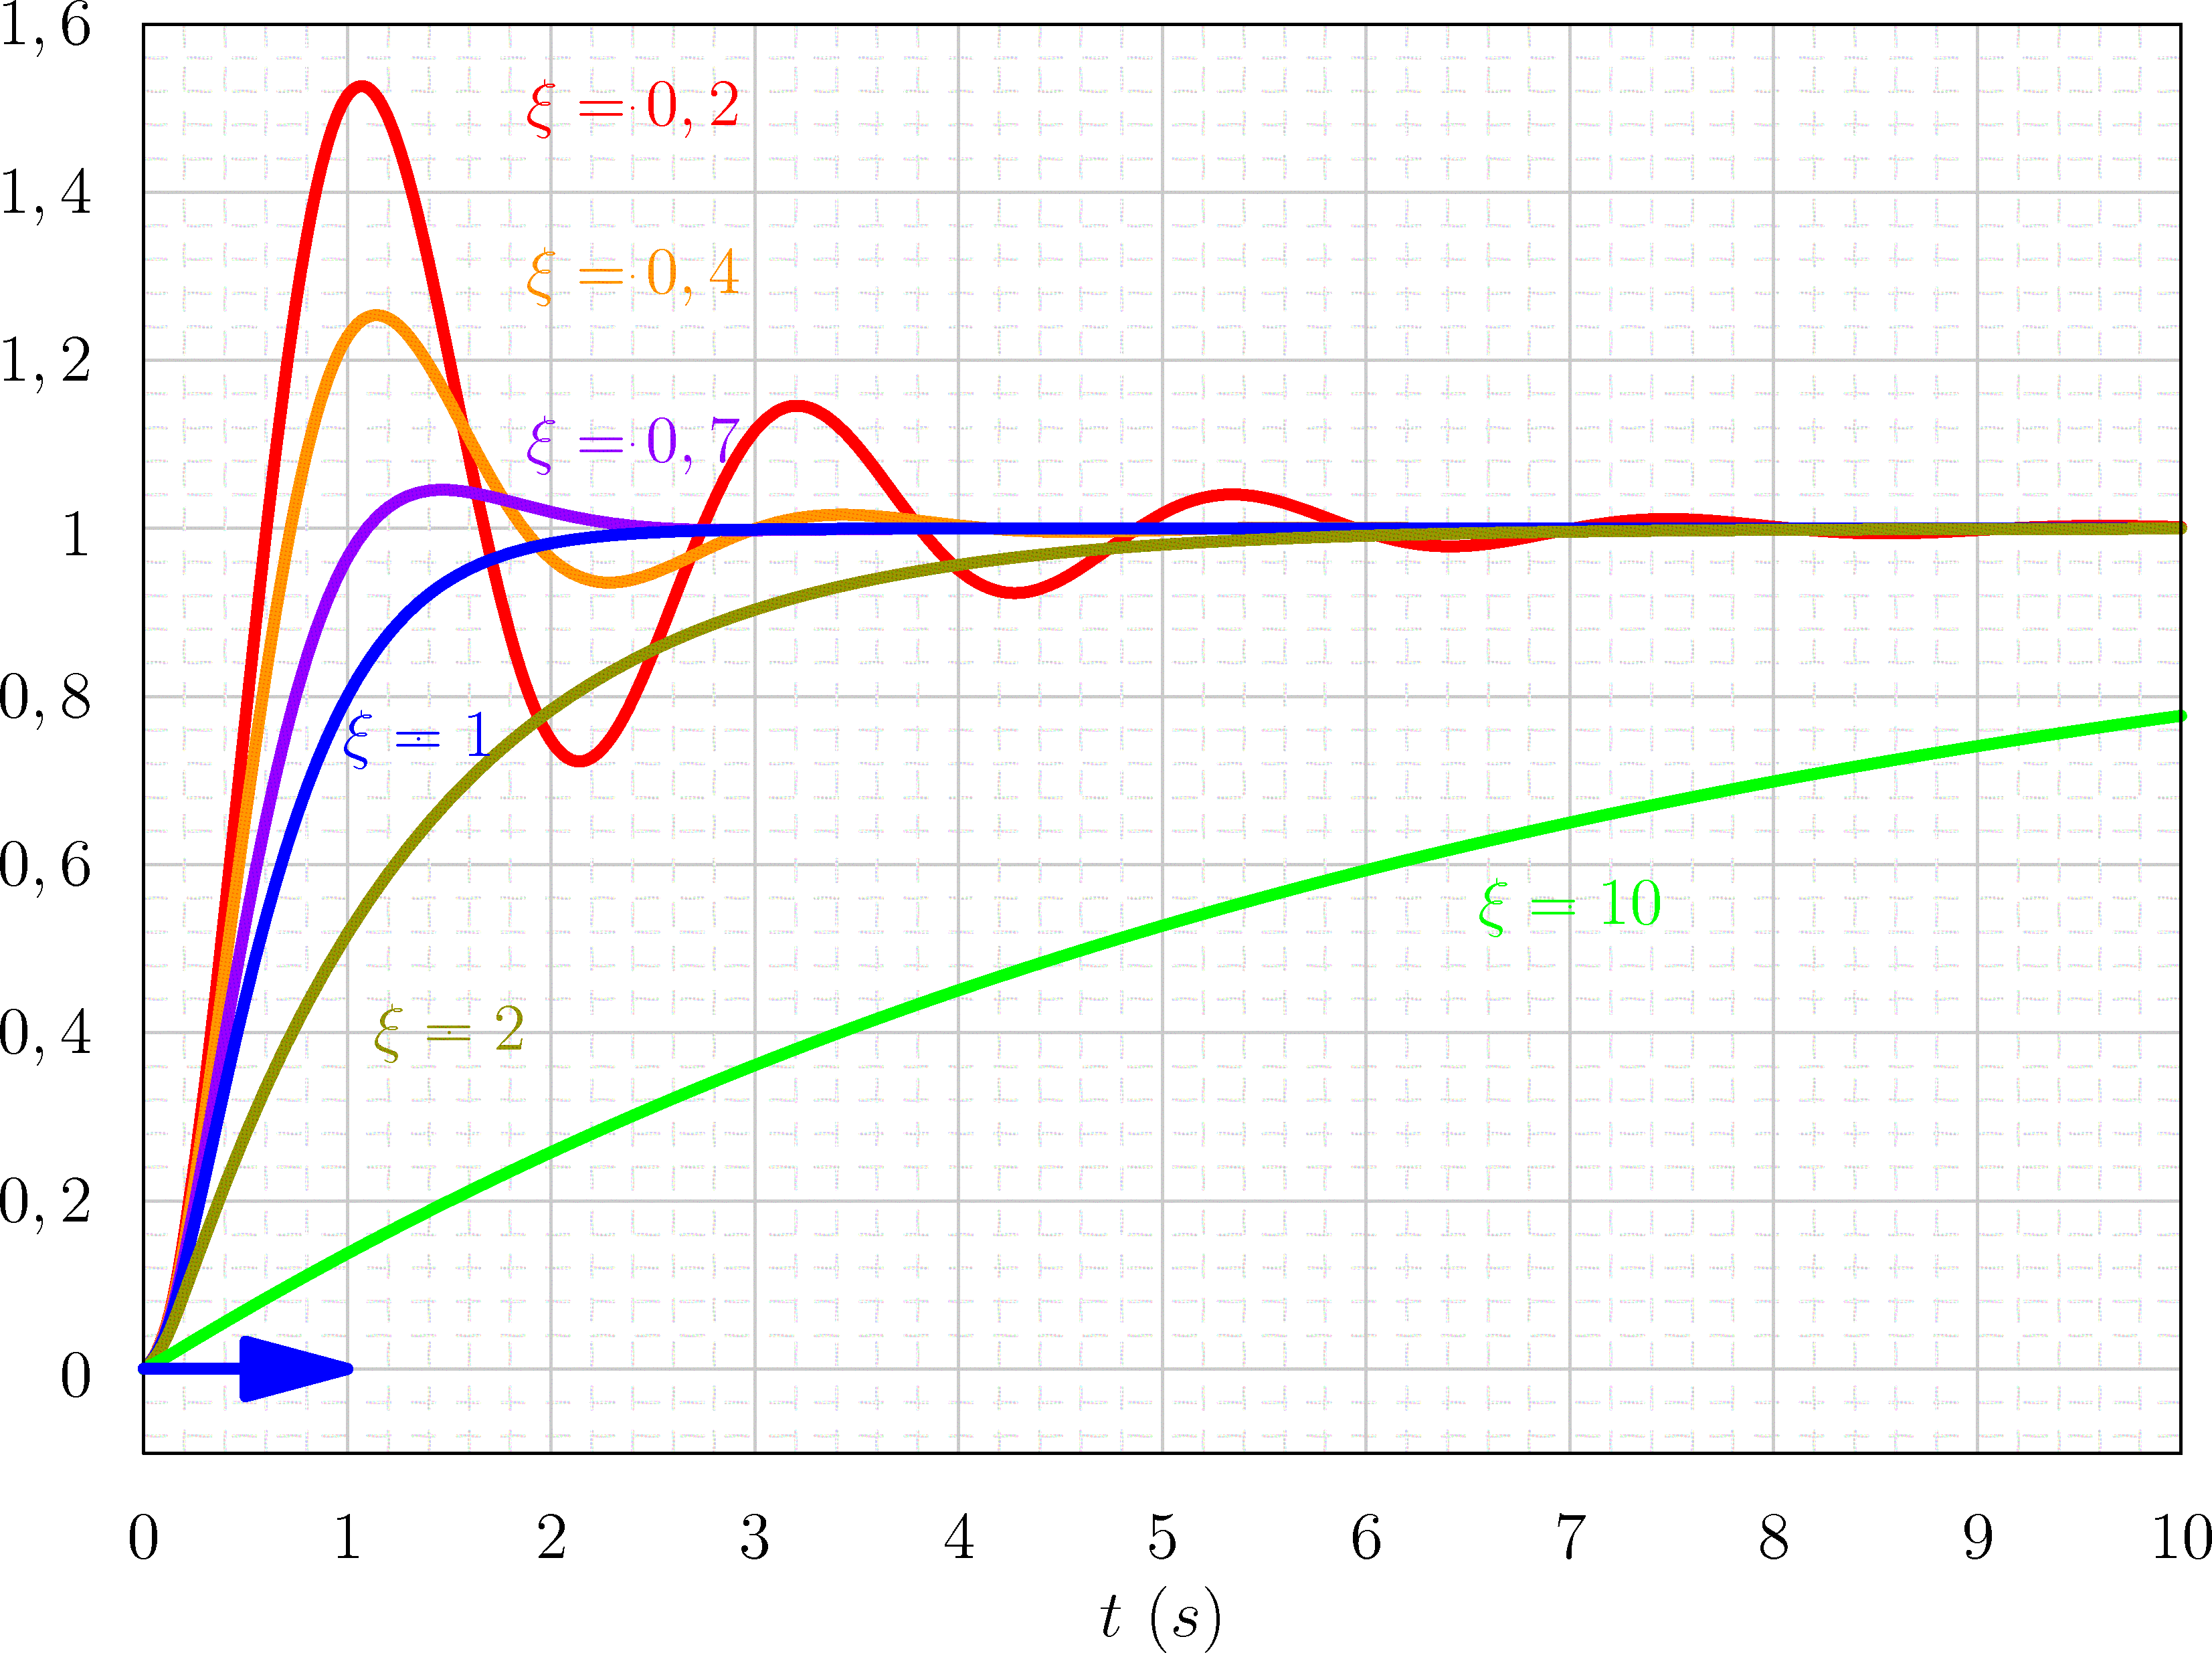
\includegraphics[width=.7\textwidth]{png/ordre2_echelon_z}

Évolution de la réponse avec les coefficient d'amortissement
\end{center}


\section{Identification des systèmes du second ordre}

        Il s’agit de déterminer, à l’aide d’essais expérimentaux, la fonction de
transfert d’un système
que l’on désire asservir. En effet, même si la structure est déterminée (sous
forme de schéma bloc),
la mise en équations est difficile (indétermination de certains paramètres,
inertie réelle, frottements,
constantes de temps, etc.).

        De plus, ces paramètres dépendent souvent des conditions dans lesquelles
sont effectuées
les mesures (atteinte de saturation, etc.). Il est donc préférable de les
déterminer dans les conditions
aussi proches que possible de l’utilisation normale du système (linéarisation
autour d’un point de
fonctionnement).

        La détermination des paramètres intervenant dans la structure s’effectue
principalement à
partir des réponses indicielles et harmoniques (traité en seconde année). On
obtient alors un
modèle dit modèle de comportement.

        L’identification sera largement abordée au cours des Travaux Pratiques.
Nous nous
limiterons, en PTSI, à l’identification de modèles d’ordre 1 ou 2, à partir de
la réponse temporelle à
une entrée type échelon.

\subsection{Système d'ordre 2 oscillant amorti}
Dans ce cas, 
$$
0<\xi<1
$$

La réponse indicielle d'un système à un échelon d'amplitude $Ec=5$ a été
enregistrée.

On obtient la courbe ci-dessous.
\begin{center}
% 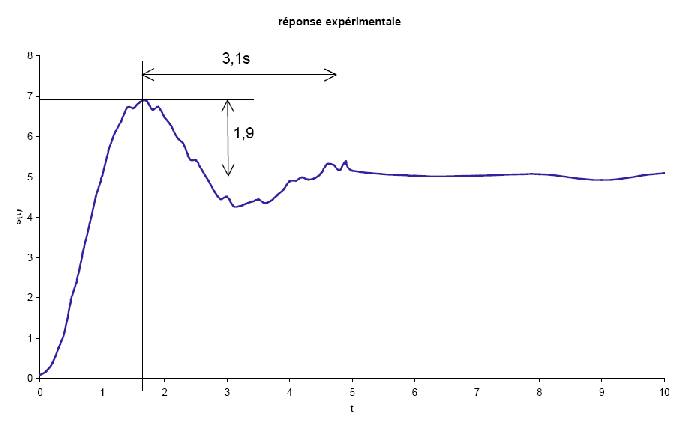
\includegraphics[width=0.7\textwidth]{png/im1}
\end{center}
Nous constatons une réponse pseudo périodique avec une pente à l’origine nulle
et des dépassements de la réponse.

\newpage

Nous adoptons pour ces raisons le modèle suivant :
$$
H(p)=\dfrac{S(p)}{E(p)}=\dfrac{K}{1+\dfrac{2\xi}{\omega_0}p+\dfrac{p^2}{
\omega_0^2}}
$$


\begin{multicols}{2}

\begin{center}
% 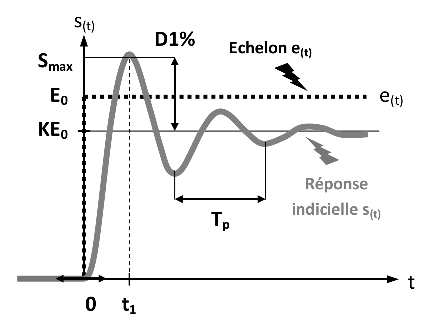
\includegraphics[width=0.4\textwidth]{png/im2}
\end{center}

\begin{center}
% 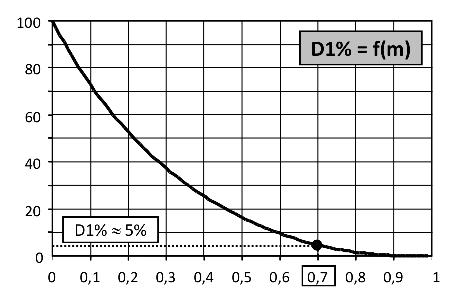
\includegraphics[width=0.4\textwidth]{eps/im3}
\end{center}

L'asymptote horizontale permet de calculer le gain statique $K$ :
$$
K=\dfrac{S_{\infty}}{E_0} \text{ où } S_{\infty} = \lim\limits_{t \to \infty}
s(t) 
$$

La réponse présente un dépassement $D_{\%}$ défini par :
$$
D_{1\%}=100 \cdot \left| \dfrac{S_{max} - S_{\infty}}{S_{\infty}} \right|
$$

Sa valeur permet de connaître le coefficient d'amortissement $\xi$ du système
car pour un système du 2\up{nd} ordre oscillant amorti on a :
$$
D_{1\%}=100 \cdot e^{\dfrac{-\pi\xi}{\sqrt{1-\xi^2}}}
$$

La courbe donne le dépassement $D_{1\%}$ en fonction de l'amortissement $\xi$. 
On peut y lire que pour $D_{1\%}\simeq 5\%$, $\xi\simeq 0,7$.

\end{multicols}

Il reste alors à déterminer la pulsation propre $\omega_0$ à partir de la
pseudo-période $T_p$ des oscillations :
$$
T_p=\dfrac{2\pi}{\omega_p}=\dfrac{2\pi}{T_P\sqrt{1-\xi^2}}
$$



En appliquant cette méthode ici, on trouve :
\begin{itemize}
 \item $K$=1
\item $\xi= 0,3$ 
\item $\omega_0=2rad/s$
\end{itemize}

La courbe réponse issue du modèle est alors tracée pour vérifier sa validité :
la fonction de transfert identifiée modélise correctement le système étudié.
\begin{center}
% 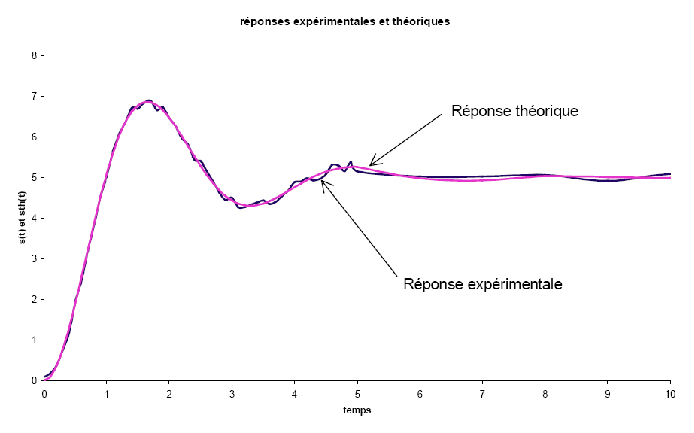
\includegraphics[width=0.7\textwidth]{eps/im4}
\end{center}

\subsection{Système d'ordre 2 non oscillant amorti}
On a donc $\xi\geq 1$.
La réponse indicielle d'un système à un échelon d'amplitude $E_c=5$ a été
enregistrée. On obtient la courbe ci-dessous.
\begin{center}
% 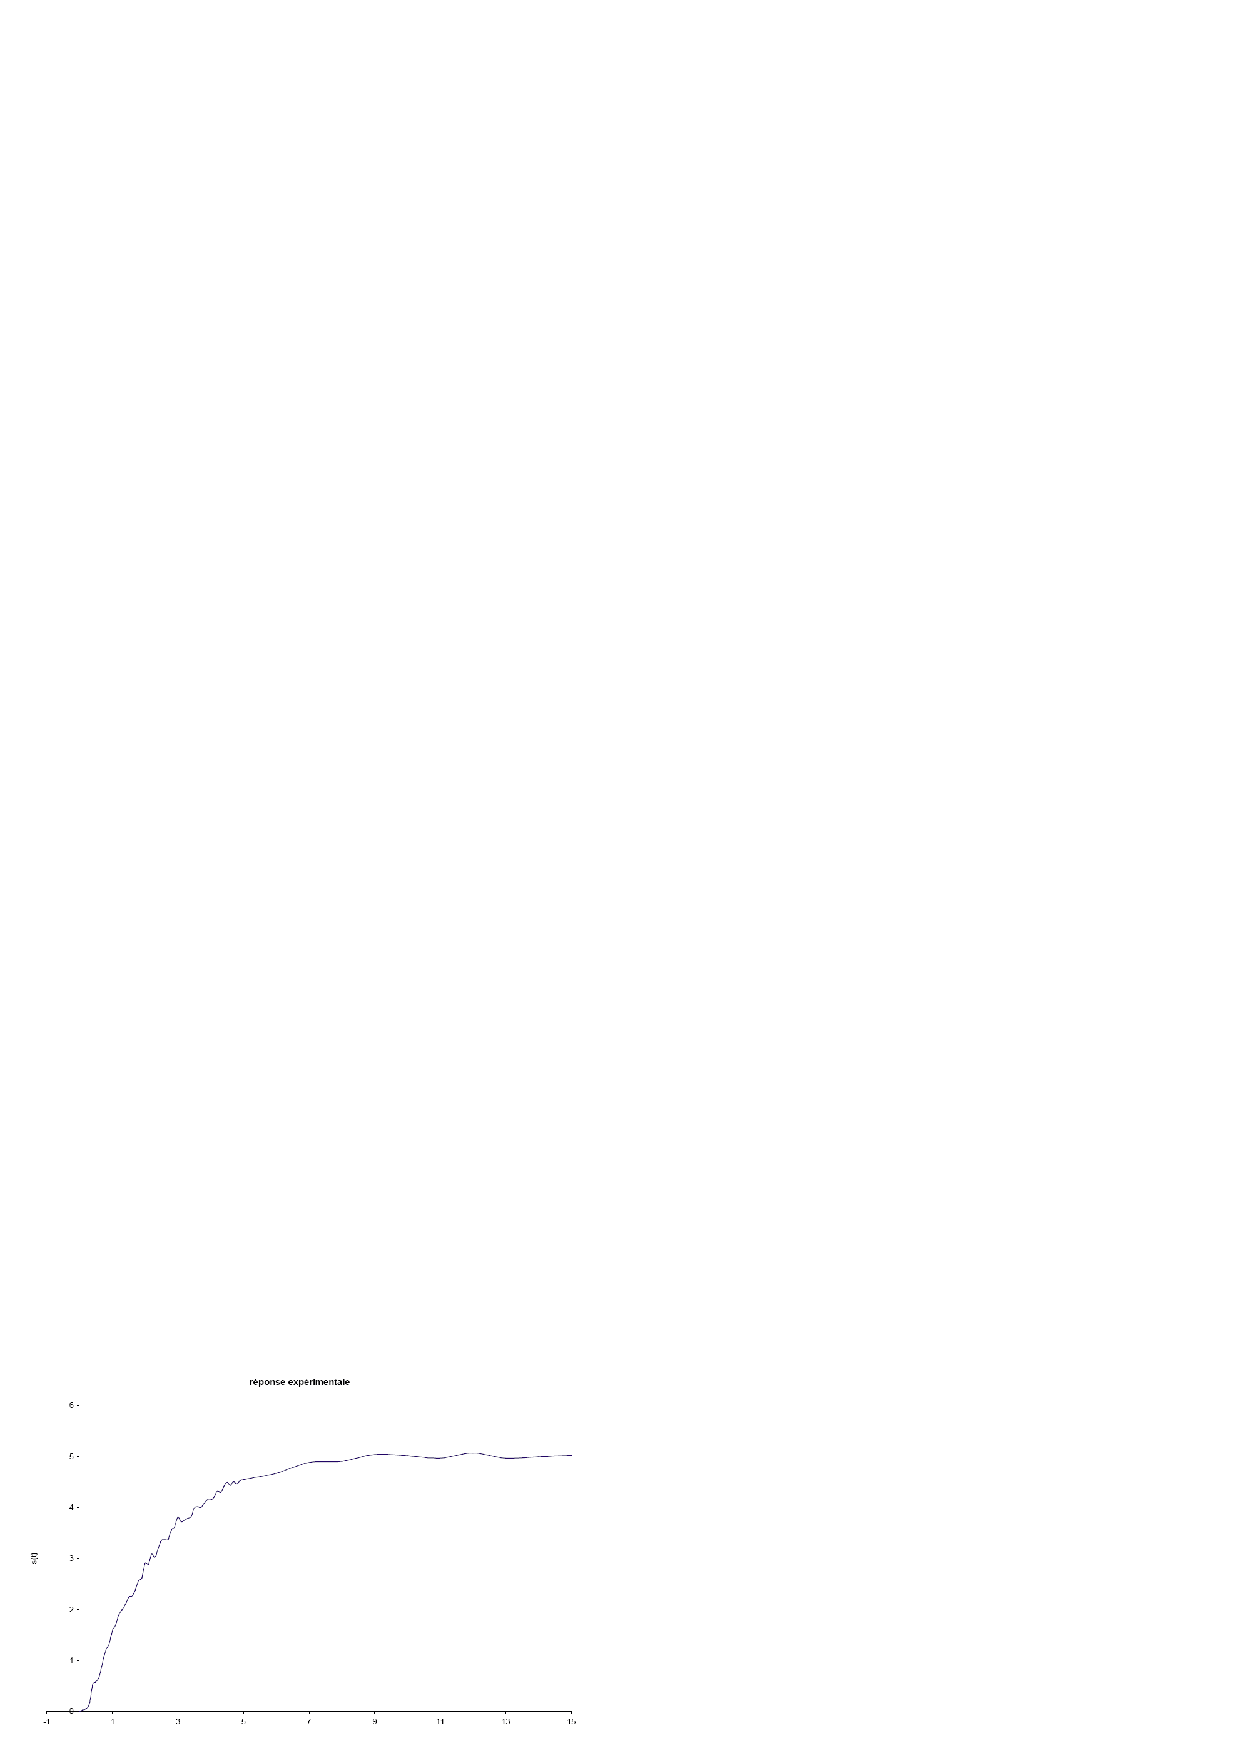
\includegraphics[width=0.7\textwidth]{eps/im5}
\end{center}

Nous constatons une réponse apériodique avec une pente à l'origine nulle et
aucun dépassement. Adoptons donc le modèle suivant : 
$$
H(p)=\dfrac{S(p)}{E(p)}=\dfrac{K}{1+\dfrac{2\xi}{\omega_0}p+\dfrac{p^2}{
\omega_0^2}}
$$

Si $\xi>1$, le système peut être considéré comme le produit de deux fonctions
de transfert du 1\up{er} ordre de constantes de temps $\tau_1$ et $\tau_2$
telles que $\tau_1>\tau_2$ :

$$
\dfrac{S(p)}{E(p)}=H(p)=\dfrac{K}{\left(1+\tau_1 p \right)\left(1+\tau_2 p
\right)}
$$

\newpage

On peut alors poser $\alpha=\tau_2/\tau_1<1$. On a donc la fonction de transfert
$H(p)$ que peut s'écrire (avec $\tau=\tau_1$):

$$
\dfrac{S(p)}{E(p)}=H(p)=\dfrac{K}{\left(1+\tau p \right)\left(1+\alpha \tau p
\right)}
$$

\begin{multicols}{2}
\begin{center}
% 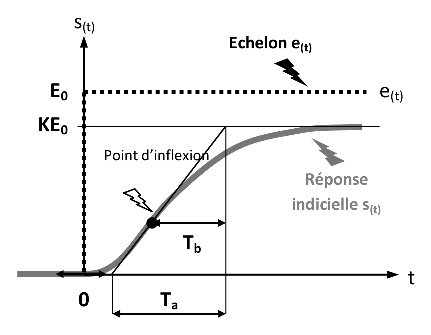
\includegraphics[width=0.4\textwidth]{eps/im6}
\end{center}

\begin{center}
 %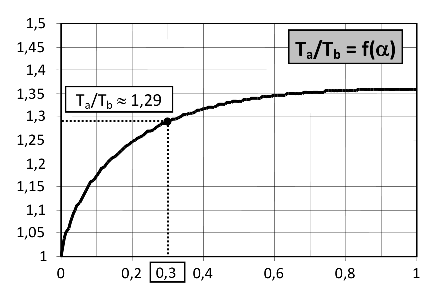
\includegraphics[width=0.4\textwidth]{eps/im7}
\end{center}

L'asymptote horizontale permet de calculer le gain statique $K$: 
$$
K=\dfrac{S_{\infty}}{E_0} \text{ où } S_{\infty} = \lim\limits_{t\to\infty} s(t)
$$

Pour déterminer les valeurs de $\alpha$ et de $\tau$, on commence par tracer la
tangente au point d'inflexion. Elle permet de définir les valeurs $T_a$ et
$T_b$. On peut démontrer que : 
$$
\dfrac{T_a}{T_b} = \dfrac{\alpha^{\dfrac{\alpha}{\alpha-1}}}{1+\alpha}
$$

La courbe correspondante tracée permet d'obtenir la valeur de $\alpha$.
Pour $\dfrac{T_a}{T_b}\simeq1,29$ on lit $\alpha\simeq 0,30$. 
La valeur de $\tau$ est donnée par :
$$
\tau = \dfrac{T_b}{1+\alpha}
$$

\end{multicols}


\end{document}
